\documentclass[mathserif,serif]{beamer}
\usepackage{tabularx}
\setbeamertemplate{footline}[frame number]
% \useoutertheme{infolines}
\usepackage{slidesphysics}
\graphicspath{{../plot/}}

\title[]{Data/MC comparison}
\author[]
{
Samuel Lo \inst{1}
\and
Yanjun Tu  \inst{1}
\and
Dongliang Zhang  \inst{2}
}
\institute[]
{
\inst{1}
The University of Hong Kong
\and
\inst{2}
University of Michigan
}
\date[]{\today}

\newcommand\Wider[2][3em]{%
\makebox[\linewidth][c]{%
\begin{minipage}{\dimexpr\textwidth+#1\relax}
\raggedright
\centering#2
\end{minipage}%
}%
}

\begin{document}
\frame{\titlepage}

\begin{frame}{Outline}
\tableofcontents
\end{frame}

\section{Update}

\begin{frame}{Update}
\begin{itemize}
\item The VV peak for nonISR\_SS\_emu is due to a large weight (1393.22) in Sherpa\_221\_NNPDF30NNLO\_lllv. \\ Solution: If the weight is larger that 100, then the weight is set to 1. \\
\url{https://twiki.cern.ch/twiki/bin/viewauth/AtlasProtected/CentralMC15ProductionList\#Treating\_high\_weights\_in\_Sherpa}
\item finished the cutflow for the signal sample
\url{https://docs.google.com/spreadsheets/d/12-hpz\_X154YYrYVbQPT6TL5JLWWPZa40NhN7AhhBpdc/edit\#gid=456557904}
\item expN for VV BG
\item Add N-1 plot for cut variables
\end{itemize}
\end{frame}

%\section{Motivation}
%\begin{frame}{Motivation}
%\begin{itemize}
%\item Optimization for signal region
%\end{itemize}
%\end{frame}

\section{CR\_SS\_run1}
\begin{frame}
\sectionpage
\end{frame}

\begin{frame}{Selection}
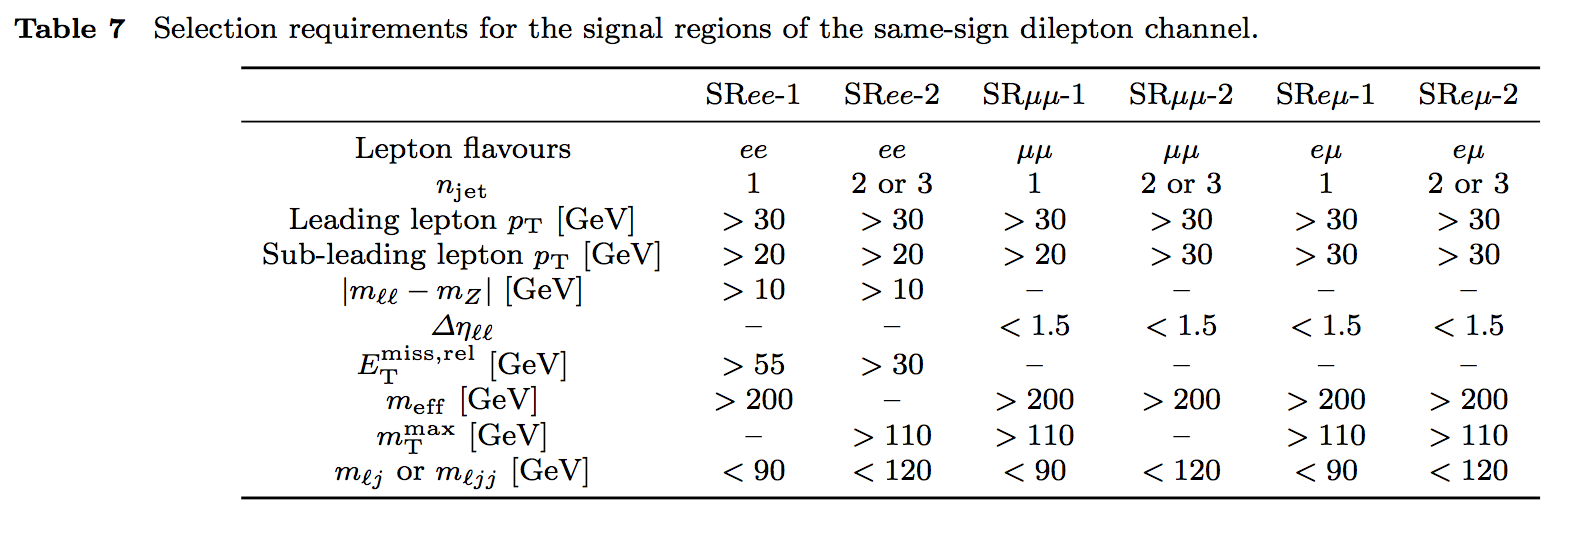
\includegraphics[width=\textwidth]{data/photo/SRcutrun1.png}
\end{frame}

\begin{frame}{Expected number of events \\ For SR\_SS\_ee\_1}
\vspace{5mm}
\begin{tabular}{|c|c|c|}
\hline
& Number of events & Significance \\
\hline
Z+jets & $18.9\pm19.8$ & \\
\hline
W+jets & $3.3\pm2.1$ & \\
\hline
top & $69.1\pm5.8$ & \\
\hline
VV & $14.1\pm2.0$ & \\
\hline
V$+\gamma$ & $12.2\pm5.5$ & \\
\hline
VVV & $0.4\pm0.1$ & \\
\hline
Total BG & $117.9\pm21.6$ & \\
\hline
Signal (175, 0) & $7.1\pm1.2$ &$-0.009$\\
\hline
Signal (165, 35) & $2.4\pm0.4$ &$-0.134$\\
\hline
Signal (400, 0) & $9.8\pm0.8$ &$0.062$\\
\hline

\end{tabular}
\end{frame}

\begin{frame}{Expected number of events \\ For SR\_SS\_mumu\_1}
\vspace{5mm}
\begin{tabular}{|c|c|c|}
\hline
& Number of events & Significance \\
\hline
Z+jets & $6.4\pm6.5$ & \\
\hline
W+jets & $0.4\pm0.4$ & \\
\hline
top & $4.0\pm0.8$ & \\
\hline
VV & $7.1\pm0.7$ & \\
\hline
V$+\gamma$ & $0.0\pm0.0$ & \\
\hline
VVV & $0.3\pm0.1$ & \\
\hline
Total BG & $18.3\pm6.6$ & \\
\hline
Signal (175, 0) & $5.4\pm0.8$ &$0.531$\\
\hline
Signal (165, 35) & $2.6\pm0.5$ &$0.159$\\
\hline
Signal (400, 0) & $9.0\pm0.9$ &$0.960$\\
\hline

\end{tabular}
\end{frame}

\begin{frame}{Expected number of events \\ For SR\_SS\_emu\_1}
\vspace{5mm}
\begin{tabular}{|c|c|c|}
\hline
& Number of events & Significance \\
\hline
Z+jets & $0.1\pm0.0$ & \\
\hline
W+jets & $5.0\pm2.4$ & \\
\hline
top & $39.9\pm3.6$ & \\
\hline
VV & $14.9\pm1.8$ & \\
\hline
V$+\gamma$ & $1.5\pm0.5$ & \\
\hline
VVV & $0.4\pm0.1$ & \\
\hline
Total BG & $61.9\pm4.7$ & \\
\hline
Signal (175, 0) & $8.1\pm1.2$ &$0.191$\\
\hline
Signal (165, 35) & $5.5\pm0.6$ &$0.068$\\
\hline
Signal (400, 0) & $15.0\pm1.1$ &$0.501$\\
\hline

\end{tabular}
\end{frame}

\begin{frame}{Expected number of events \\ For SR\_SS\_ee\_2}
\vspace{5mm}
\begin{tabular}{|c|c|c|}
\hline
& Number of events & Significance \\
\hline
VV & $2.8\pm0.4$ & \\
\hline
V$+\gamma$ & $2.3\pm1.2$ & \\
\hline
Total BG & $5.1\pm1.2$ & \\
\hline
Signal (400, 380) & $0.0\pm0.0$ &$-0.229$\\
\hline
Signal (500, 450) & $0.1\pm0.0$ &$-0.188$\\
\hline
Signal (400, 300) & $0.8\pm0.1$ &$0.045$\\
\hline
Signal (400, 200) & $0.5\pm0.1$ &$-0.040$\\
\hline
Signal (400, 100) & $0.4\pm0.2$ &$-0.088$\\
\hline

\end{tabular}
\end{frame}

\begin{frame}{Expected number of events \\ For SR\_SS\_mumu\_2}
\vspace{5mm}
\begin{tabular}{|c|c|c|}
\hline
& Number of events & Significance \\
\hline
Z+jets & $89.3\pm27.3$ & \\
\hline
W+jets & $1.1\pm0.6$ & \\
\hline
top & $10.7\pm1.5$ & \\
\hline
VV & $16.3\pm0.7$ & \\
\hline
V$+\gamma$ & $2.5\pm1.3$ & \\
\hline
VVV & $0.3\pm0.1$ & \\
\hline
Total BG & $120.1\pm27.4$ & \\
\hline
Signal (175, 0) & $9.7\pm1.3$ &$0.055$\\
\hline
Signal (165, 35) & $4.1\pm0.5$ &$-0.091$\\
\hline
Signal (400, 0) & $7.5\pm0.7$ &$-0.003$\\
\hline

\end{tabular}
\end{frame}

\begin{frame}{Expected number of events \\ For SR\_SS\_emu\_2}
\vspace{5mm}
\begin{tabular}{|c|c|c|}
\hline
& Number of events & Significance \\
\hline
VV & $6.0\pm0.4$ & \\
\hline
V$+\gamma$ & $1.1\pm0.8$ & \\
\hline
Total BG & $7.1\pm0.9$ & \\
\hline
Signal (400, 380) & $0.0\pm0.0$ &$-0.213$\\
\hline
Signal (500, 450) & $0.2\pm0.0$ &$-0.162$\\
\hline
Signal (400, 300) & $1.3\pm0.2$ &$0.163$\\
\hline
Signal (400, 200) & $0.8\pm0.1$ &$0.014$\\
\hline
Signal (400, 100) & $0.5\pm0.2$ &$-0.075$\\
\hline

\end{tabular}
\end{frame}



\begin{frame}{Selection}
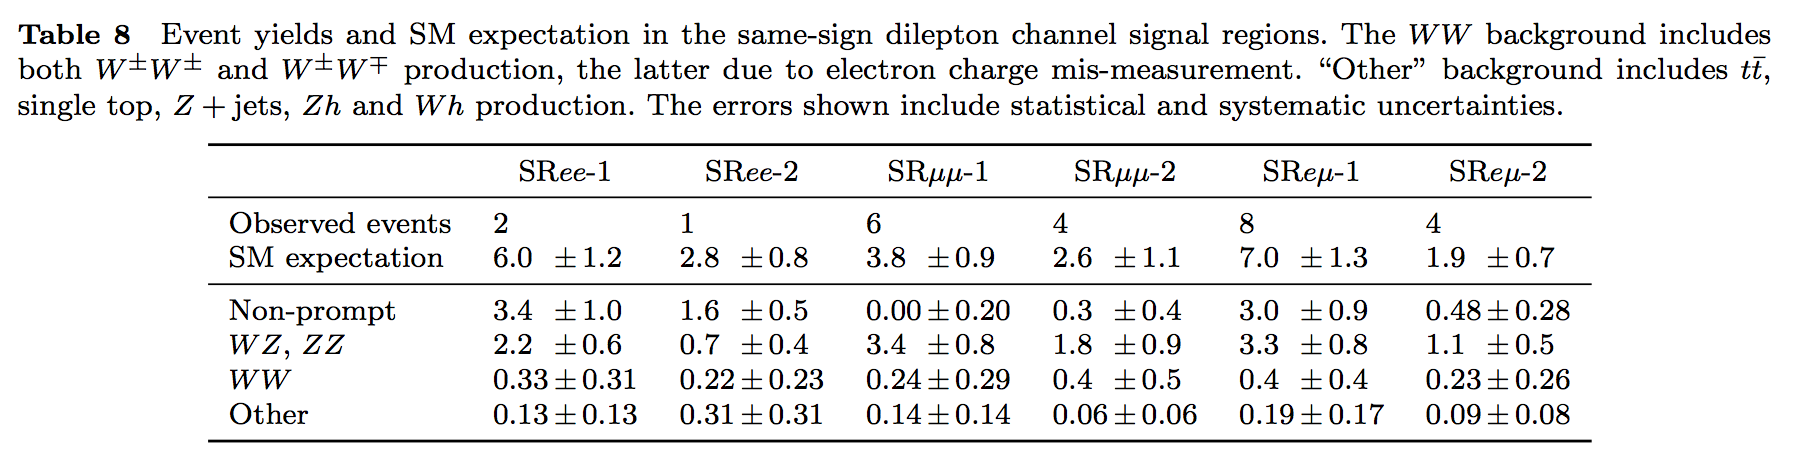
\includegraphics[width=\textwidth]{data/photo/expNrun1.png}
\end{frame}

\begin{frame}{Expected number of events for VV \\ For SR\_SS\_ee\_1}
\vspace{5mm}
\begin{tabular}{|c|c|}
\hline
& Number of events \\
\hline
Sherpa\_221\_NNPDF30NNLO\_llll & $0.081\pm0.022$ \\
\hline
Sherpa\_221\_NNPDF30NNLO\_lllv & $7.680\pm0.780$ \\
\hline
Sherpa\_221\_NNPDF30NNLO\_llvv & $4.995\pm1.087$ \\
\hline
Sherpa\_CT10\_llvvjj\_ss\_EW4 & $0.249\pm0.024$ \\
\hline
Sherpa\_CT10\_llvvjj\_ss\_EW6 & $0.890\pm0.051$ \\
\hline
Sherpa\_CT10\_lllvjj\_EW6 & $0.001\pm0.000$ \\
\hline
Sherpa\_CT10\_lllljj\_EW6 & $0.000\pm0.000$ \\
\hline
Sherpa\_CT10\_ggllll & $0.009\pm0.006$ \\
\hline
Sherpa\_CT10\_ggllvv & $0.000\pm0.000$ \\
\hline
Sherpa\_221\_NNPDF30NNLO\_ZqqZll & $0.000\pm0.000$ \\
\hline
Sherpa\_221\_NNPDF30NNLO\_WqqZll & $-0.030\pm0.042$ \\
\hline

\end{tabular}
\end{frame}

\begin{frame}{Expected number of events for VV \\ For SR\_SS\_mumu\_1}
\vspace{5mm}
\begin{tabular}{|c|c|}
\hline
& Number of events \\
\hline
Sherpa\_221\_NNPDF30NNLO\_llll & $0.178\pm0.037$ \\
\hline
Sherpa\_221\_NNPDF30NNLO\_lllv & $5.509\pm0.689$ \\
\hline
Sherpa\_221\_NNPDF30NNLO\_llvv & $0.178\pm0.098$ \\
\hline
Sherpa\_CT10\_llvvjj\_ss\_EW4 & $0.136\pm0.016$ \\
\hline
Sherpa\_CT10\_llvvjj\_ss\_EW6 & $0.800\pm0.053$ \\
\hline
Sherpa\_CT10\_lllvjj\_EW6 & $0.000\pm0.000$ \\
\hline
Sherpa\_CT10\_lllljj\_EW6 & $0.005\pm0.005$ \\
\hline
Sherpa\_CT10\_ggllll & $0.022\pm0.011$ \\
\hline
Sherpa\_CT10\_ggllvv & $0.000\pm0.000$ \\
\hline
Sherpa\_221\_NNPDF30NNLO\_ZqqZll & $0.000\pm0.000$ \\
\hline
Sherpa\_221\_NNPDF30NNLO\_WqqZll & $0.000\pm0.000$ \\
\hline

\end{tabular}
\end{frame}

\begin{frame}{Expected number of events for VV \\ For SR\_SS\_emu\_1}
\vspace{5mm}
\begin{tabular}{|c|c|}
\hline
& Number of events \\
\hline
Sherpa\_221\_NNPDF30NNLO\_llll & $0.193\pm0.057$ \\
\hline
Sherpa\_221\_NNPDF30NNLO\_lllv & $8.253\pm0.704$ \\
\hline
Sherpa\_221\_NNPDF30NNLO\_llvv & $1.230\pm0.432$ \\
\hline
Sherpa\_CT10\_llvvjj\_ss\_EW4 & $0.166\pm0.016$ \\
\hline
Sherpa\_CT10\_llvvjj\_ss\_EW6 & $1.174\pm0.059$ \\
\hline
Sherpa\_CT10\_lllvjj\_EW6 & $0.001\pm0.000$ \\
\hline
Sherpa\_CT10\_lllljj\_EW6 & $0.000\pm0.000$ \\
\hline
Sherpa\_CT10\_ggllll & $0.014\pm0.004$ \\
\hline
Sherpa\_CT10\_ggllvv & $0.085\pm0.085$ \\
\hline
Sherpa\_221\_NNPDF30NNLO\_ZqqZll & $0.000\pm0.000$ \\
\hline
Sherpa\_221\_NNPDF30NNLO\_WqqZll & $0.000\pm0.000$ \\
\hline

\end{tabular}
\end{frame}

\begin{frame}{Expected number of events for VV \\ For SR\_SS\_ee\_2}
\vspace{5mm}
\begin{tabular}{|c|c|}
\hline
& Number of events \\
\hline
Sherpa\_221\_NNPDF30NNLO\_llll & $-0.033\pm0.024$ \\
\hline
Sherpa\_221\_NNPDF30NNLO\_lllv & $1.624\pm0.270$ \\
\hline
Sherpa\_221\_NNPDF30NNLO\_llvv & $0.524\pm0.266$ \\
\hline
Sherpa\_CT10\_llvvjj\_ss\_EW4 & $0.115\pm0.015$ \\
\hline
Sherpa\_CT10\_llvvjj\_ss\_EW6 & $0.556\pm0.046$ \\
\hline
Sherpa\_CT10\_lllvjj\_EW6 & $0.000\pm0.000$ \\
\hline
Sherpa\_CT10\_lllljj\_EW6 & $0.000\pm0.000$ \\
\hline
Sherpa\_CT10\_ggllll & $0.003\pm0.002$ \\
\hline
Sherpa\_CT10\_ggllvv & $0.000\pm0.000$ \\
\hline
Sherpa\_221\_NNPDF30NNLO\_ZqqZll & $0.000\pm0.000$ \\
\hline
Sherpa\_221\_NNPDF30NNLO\_WqqZll & $0.000\pm0.000$ \\
\hline

\end{tabular}
\end{frame}

\begin{frame}{Expected number of events for VV \\ For SR\_SS\_mumu\_2}
\vspace{5mm}
\begin{tabular}{|c|c|}
\hline
& Number of events \\
\hline
Sherpa\_221\_NNPDF30NNLO\_llll & $0.915\pm0.097$ \\
\hline
Sherpa\_221\_NNPDF30NNLO\_lllv & $11.974\pm0.605$ \\
\hline
Sherpa\_221\_NNPDF30NNLO\_llvv & $0.292\pm0.154$ \\
\hline
Sherpa\_CT10\_llvvjj\_ss\_EW4 & $0.328\pm0.031$ \\
\hline
Sherpa\_CT10\_llvvjj\_ss\_EW6 & $2.423\pm0.097$ \\
\hline
Sherpa\_CT10\_lllvjj\_EW6 & $0.001\pm0.000$ \\
\hline
Sherpa\_CT10\_lllljj\_EW6 & $0.019\pm0.009$ \\
\hline
Sherpa\_CT10\_ggllll & $0.055\pm0.009$ \\
\hline
Sherpa\_CT10\_ggllvv & $0.000\pm0.000$ \\
\hline
Sherpa\_221\_NNPDF30NNLO\_ZqqZll & $0.280\pm0.103$ \\
\hline
Sherpa\_221\_NNPDF30NNLO\_WqqZll & $0.284\pm0.123$ \\
\hline

\end{tabular}
\end{frame}

\begin{frame}{Expected number of events for VV \\ For SR\_SS\_emu\_2}
\vspace{5mm}
\begin{tabular}{|c|c|}
\hline
& Number of events \\
\hline
Sherpa\_221\_NNPDF30NNLO\_llll & $0.134\pm0.032$ \\
\hline
Sherpa\_221\_NNPDF30NNLO\_lllv & $4.017\pm0.377$ \\
\hline
Sherpa\_221\_NNPDF30NNLO\_llvv & $0.501\pm0.197$ \\
\hline
Sherpa\_CT10\_llvvjj\_ss\_EW4 & $0.126\pm0.016$ \\
\hline
Sherpa\_CT10\_llvvjj\_ss\_EW6 & $1.200\pm0.062$ \\
\hline
Sherpa\_CT10\_lllvjj\_EW6 & $0.001\pm0.000$ \\
\hline
Sherpa\_CT10\_lllljj\_EW6 & $0.000\pm0.000$ \\
\hline
Sherpa\_CT10\_ggllll & $0.009\pm0.004$ \\
\hline
Sherpa\_CT10\_ggllvv & $0.000\pm0.000$ \\
\hline
Sherpa\_221\_NNPDF30NNLO\_ZqqZll & $0.000\pm0.000$ \\
\hline
Sherpa\_221\_NNPDF30NNLO\_WqqZll & $0.000\pm0.000$ \\
\hline

\end{tabular}
\end{frame}


\begin{frame}{For SR\_SS\_run1 \\ $\pt$ of the leading lepton}
\Wider[5em]{
\includegraphics[width=0.33\textwidth]{pt1_SR_SS_ee_1}
\includegraphics[width=0.33\textwidth]{pt1_SR_SS_mumu_1}
\includegraphics[width=0.33\textwidth]{pt1_SR_SS_emu_1} \\
\includegraphics[width=0.33\textwidth]{pt1_SR_SS_ee_2}
\includegraphics[width=0.33\textwidth]{pt1_SR_SS_mumu_2}
\includegraphics[width=0.33\textwidth]{pt1_SR_SS_emu_2}
}
\end{frame}

\begin{frame}{For SR\_SS\_run1 \\ $\pt$ of the subleading lepton}
\Wider[5em]{
\includegraphics[width=0.33\textwidth]{pt2_SR_SS_ee_1}
\includegraphics[width=0.33\textwidth]{pt2_SR_SS_mumu_1}
\includegraphics[width=0.33\textwidth]{pt2_SR_SS_emu_1} \\
\includegraphics[width=0.33\textwidth]{pt2_SR_SS_ee_2}
\includegraphics[width=0.33\textwidth]{pt2_SR_SS_mumu_2}
\includegraphics[width=0.33\textwidth]{pt2_SR_SS_emu_2}
}
\end{frame}

\begin{frame}{For SR\_SS\_run1 \\ $\eta$ of the leading lepton}
\Wider[5em]{
\includegraphics[width=0.33\textwidth]{eta1_SR_SS_ee_1}
\includegraphics[width=0.33\textwidth]{eta1_SR_SS_mumu_1}
\includegraphics[width=0.33\textwidth]{eta1_SR_SS_emu_1} \\
\includegraphics[width=0.33\textwidth]{eta1_SR_SS_ee_2}
\includegraphics[width=0.33\textwidth]{eta1_SR_SS_mumu_2}
\includegraphics[width=0.33\textwidth]{eta1_SR_SS_emu_2}
}
\end{frame}

\begin{frame}{For SR\_SS\_run1 \\ $\eta$ of the subleading lepton}
\Wider[5em]{
\includegraphics[width=0.33\textwidth]{eta2_SR_SS_ee_1}
\includegraphics[width=0.33\textwidth]{eta2_SR_SS_mumu_1}
\includegraphics[width=0.33\textwidth]{eta2_SR_SS_emu_1} \\
\includegraphics[width=0.33\textwidth]{eta2_SR_SS_ee_2}
\includegraphics[width=0.33\textwidth]{eta2_SR_SS_mumu_2}
\includegraphics[width=0.33\textwidth]{eta2_SR_SS_emu_2}
}
\end{frame}

\begin{frame}{For SR\_SS\_run1 \\ $\phi$ of the leading lepton}
\Wider[5em]{
\includegraphics[width=0.33\textwidth]{phi1_SR_SS_ee_1}
\includegraphics[width=0.33\textwidth]{phi1_SR_SS_mumu_1}
\includegraphics[width=0.33\textwidth]{phi1_SR_SS_emu_1} \\
\includegraphics[width=0.33\textwidth]{phi1_SR_SS_ee_2}
\includegraphics[width=0.33\textwidth]{phi1_SR_SS_mumu_2}
\includegraphics[width=0.33\textwidth]{phi1_SR_SS_emu_2}
}
\end{frame}

\begin{frame}{For SR\_SS\_run1 \\ $m_{ll}$}
\Wider[5em]{
\includegraphics[width=0.33\textwidth]{mll_SR_SS_ee_1}
\includegraphics[width=0.33\textwidth]{mll_SR_SS_mumu_1}
\includegraphics[width=0.33\textwidth]{mll_SR_SS_emu_1} \\
\includegraphics[width=0.33\textwidth]{mll_SR_SS_ee_2}
\includegraphics[width=0.33\textwidth]{mll_SR_SS_mumu_2}
\includegraphics[width=0.33\textwidth]{mll_SR_SS_emu_2}
}
\end{frame}

\begin{frame}{For SR\_SS\_run1 \\ Dilepton $\pt$}
\Wider[5em]{
\includegraphics[width=0.33\textwidth]{ptll_SR_SS_ee_1}
\includegraphics[width=0.33\textwidth]{ptll_SR_SS_mumu_1}
\includegraphics[width=0.33\textwidth]{ptll_SR_SS_emu_1} \\
\includegraphics[width=0.33\textwidth]{ptll_SR_SS_ee_2}
\includegraphics[width=0.33\textwidth]{ptll_SR_SS_mumu_2}
\includegraphics[width=0.33\textwidth]{ptll_SR_SS_emu_2}
}
\end{frame}

\begin{frame}{For SR\_SS\_run1 \\ $E_{\text{T}}^{\text{miss}}$}
\Wider[5em]{
\includegraphics[width=0.33\textwidth]{MET_SR_SS_ee_1}
\includegraphics[width=0.33\textwidth]{MET_SR_SS_mumu_1}
\includegraphics[width=0.33\textwidth]{MET_SR_SS_emu_1} \\
\includegraphics[width=0.33\textwidth]{MET_SR_SS_ee_2}
\includegraphics[width=0.33\textwidth]{MET_SR_SS_mumu_2}
\includegraphics[width=0.33\textwidth]{MET_SR_SS_emu_2}
}
\end{frame}

\begin{frame}{For SR\_SS\_run1 \\ $m_{T2}$}
\Wider[5em]{
\includegraphics[width=0.33\textwidth]{mTtwo_SR_SS_ee_1}
\includegraphics[width=0.33\textwidth]{mTtwo_SR_SS_mumu_1}
\includegraphics[width=0.33\textwidth]{mTtwo_SR_SS_emu_1} \\
\includegraphics[width=0.33\textwidth]{mTtwo_SR_SS_ee_2}
\includegraphics[width=0.33\textwidth]{mTtwo_SR_SS_mumu_2}
\includegraphics[width=0.33\textwidth]{mTtwo_SR_SS_emu_2}
}
\end{frame}

\begin{frame}{For SR\_SS\_run1 \\ $m_{\text{T}}$ of the leading lepton}
\Wider[5em]{
\includegraphics[width=0.33\textwidth]{mt1_SR_SS_ee_1}
\includegraphics[width=0.33\textwidth]{mt1_SR_SS_mumu_1}
\includegraphics[width=0.33\textwidth]{mt1_SR_SS_emu_1} \\
\includegraphics[width=0.33\textwidth]{mt1_SR_SS_ee_2}
\includegraphics[width=0.33\textwidth]{mt1_SR_SS_mumu_2}
\includegraphics[width=0.33\textwidth]{mt1_SR_SS_emu_2}
}
\end{frame}

\begin{frame}{For SR\_SS\_run1 \\ $m_{\text{T}}$ of the subleading lepton}
\Wider[5em]{
\includegraphics[width=0.33\textwidth]{mt2_SR_SS_ee_1}
\includegraphics[width=0.33\textwidth]{mt2_SR_SS_mumu_1}
\includegraphics[width=0.33\textwidth]{mt2_SR_SS_emu_1} \\
\includegraphics[width=0.33\textwidth]{mt2_SR_SS_ee_2}
\includegraphics[width=0.33\textwidth]{mt2_SR_SS_mumu_2}
\includegraphics[width=0.33\textwidth]{mt2_SR_SS_emu_2}
}
\end{frame}

\begin{frame}{For SR\_SS\_run1 \\ $\pt$ of the leading jet}
\Wider[5em]{
\includegraphics[width=0.33\textwidth]{jetpt_SR_SS_ee_1}
\includegraphics[width=0.33\textwidth]{jetpt_SR_SS_mumu_1}
\includegraphics[width=0.33\textwidth]{jetpt_SR_SS_emu_1} \\
\includegraphics[width=0.33\textwidth]{jetpt_SR_SS_ee_2}
\includegraphics[width=0.33\textwidth]{jetpt_SR_SS_mumu_2}
\includegraphics[width=0.33\textwidth]{jetpt_SR_SS_emu_2}
}
\end{frame}

\begin{frame}{For SR\_SS\_run1 \\ $\eta$ of the leading jet}
\Wider[5em]{
\includegraphics[width=0.33\textwidth]{jeteta_SR_SS_ee_1}
\includegraphics[width=0.33\textwidth]{jeteta_SR_SS_mumu_1}
\includegraphics[width=0.33\textwidth]{jeteta_SR_SS_emu_1} \\
\includegraphics[width=0.33\textwidth]{jeteta_SR_SS_ee_2}
\includegraphics[width=0.33\textwidth]{jeteta_SR_SS_mumu_2}
\includegraphics[width=0.33\textwidth]{jeteta_SR_SS_emu_2}
}
\end{frame}

\begin{frame}{For SR\_SS\_run1 \\ Number of jets}
\Wider[5em]{
\includegraphics[width=0.33\textwidth]{nJet_SR_SS_ee_1}
\includegraphics[width=0.33\textwidth]{nJet_SR_SS_mumu_1}
\includegraphics[width=0.33\textwidth]{nJet_SR_SS_emu_1} \\
\includegraphics[width=0.33\textwidth]{nJet_SR_SS_ee_2}
\includegraphics[width=0.33\textwidth]{nJet_SR_SS_mumu_2}
\includegraphics[width=0.33\textwidth]{nJet_SR_SS_emu_2}
}
\end{frame}

\begin{frame}{For SR\_SS\_run1 \\ Number of b-jets}
\Wider[5em]{
\includegraphics[width=0.33\textwidth]{nBJet_SR_SS_ee_1}
\includegraphics[width=0.33\textwidth]{nBJet_SR_SS_mumu_1}
\includegraphics[width=0.33\textwidth]{nBJet_SR_SS_emu_1} \\
\includegraphics[width=0.33\textwidth]{nBJet_SR_SS_ee_2}
\includegraphics[width=0.33\textwidth]{nBJet_SR_SS_mumu_2}
\includegraphics[width=0.33\textwidth]{nBJet_SR_SS_emu_2}
}
\end{frame}

\begin{frame}{For SR\_SS\_run1 \\ Number of central jets}
\Wider[5em]{
\includegraphics[width=0.33\textwidth]{nCJet_SR_SS_ee_1}
\includegraphics[width=0.33\textwidth]{nCJet_SR_SS_mumu_1}
\includegraphics[width=0.33\textwidth]{nCJet_SR_SS_emu_1} \\
\includegraphics[width=0.33\textwidth]{nCJet_SR_SS_ee_2}
\includegraphics[width=0.33\textwidth]{nCJet_SR_SS_mumu_2}
\includegraphics[width=0.33\textwidth]{nCJet_SR_SS_emu_2}
}
\end{frame}

\begin{frame}{For SR\_SS\_run1 \\ $\Delta\phi_{ll}$}
\Wider[5em]{
\includegraphics[width=0.33\textwidth]{l12_dPhi_SR_SS_ee_1}
\includegraphics[width=0.33\textwidth]{l12_dPhi_SR_SS_mumu_1}
\includegraphics[width=0.33\textwidth]{l12_dPhi_SR_SS_emu_1} \\
\includegraphics[width=0.33\textwidth]{l12_dPhi_SR_SS_ee_2}
\includegraphics[width=0.33\textwidth]{l12_dPhi_SR_SS_mumu_2}
\includegraphics[width=0.33\textwidth]{l12_dPhi_SR_SS_emu_2}
}
\end{frame}

\begin{frame}{For SR\_SS\_run1 \\ $\Delta\phi_{ll,\text{MET}}$}
\Wider[5em]{
\includegraphics[width=0.33\textwidth]{l12_MET_dPhi_SR_SS_ee_1}
\includegraphics[width=0.33\textwidth]{l12_MET_dPhi_SR_SS_mumu_1}
\includegraphics[width=0.33\textwidth]{l12_MET_dPhi_SR_SS_emu_1} \\
\includegraphics[width=0.33\textwidth]{l12_MET_dPhi_SR_SS_ee_2}
\includegraphics[width=0.33\textwidth]{l12_MET_dPhi_SR_SS_mumu_2}
\includegraphics[width=0.33\textwidth]{l12_MET_dPhi_SR_SS_emu_2}
}
\end{frame}

\begin{frame}{For SR\_SS\_run1 \\ $\Delta\phi_{\text{jet0,MET}}$}
\Wider[5em]{
\includegraphics[width=0.33\textwidth]{jets_MET_dPhi_SR_SS_ee_1}
\includegraphics[width=0.33\textwidth]{jets_MET_dPhi_SR_SS_mumu_1}
\includegraphics[width=0.33\textwidth]{jets_MET_dPhi_SR_SS_emu_1} \\
\includegraphics[width=0.33\textwidth]{jets_MET_dPhi_SR_SS_ee_2}
\includegraphics[width=0.33\textwidth]{jets_MET_dPhi_SR_SS_mumu_2}
\includegraphics[width=0.33\textwidth]{jets_MET_dPhi_SR_SS_emu_2}
}
\end{frame}

\begin{frame}{For SR\_SS\_run1 \\ $\Delta\eta_{ll}$}
\Wider[5em]{
\includegraphics[width=0.33\textwidth]{dEta_SR_SS_ee_1}
\includegraphics[width=0.33\textwidth]{dEta_SR_SS_mumu_1}
\includegraphics[width=0.33\textwidth]{dEta_SR_SS_emu_1} \\
\includegraphics[width=0.33\textwidth]{dEta_SR_SS_ee_2}
\includegraphics[width=0.33\textwidth]{dEta_SR_SS_mumu_2}
\includegraphics[width=0.33\textwidth]{dEta_SR_SS_emu_2}
}
\end{frame}

\begin{frame}{For SR\_SS\_run1 \\ $E_{\text{T}}^{\text{miss,rel}}$}
\Wider[5em]{
\includegraphics[width=0.33\textwidth]{METRel_SR_SS_ee_1}
\includegraphics[width=0.33\textwidth]{METRel_SR_SS_mumu_1}
\includegraphics[width=0.33\textwidth]{METRel_SR_SS_emu_1} \\
\includegraphics[width=0.33\textwidth]{METRel_SR_SS_ee_2}
\includegraphics[width=0.33\textwidth]{METRel_SR_SS_mumu_2}
\includegraphics[width=0.33\textwidth]{METRel_SR_SS_emu_2}
}
\end{frame}

\begin{frame}{For SR\_SS\_run1 \\ $m_{\text{eff}}$}
\Wider[5em]{
\includegraphics[width=0.33\textwidth]{meff_SR_SS_ee_1}
\includegraphics[width=0.33\textwidth]{meff_SR_SS_mumu_1}
\includegraphics[width=0.33\textwidth]{meff_SR_SS_emu_1} \\
\includegraphics[width=0.33\textwidth]{meff_SR_SS_ee_2}
\includegraphics[width=0.33\textwidth]{meff_SR_SS_mumu_2}
\includegraphics[width=0.33\textwidth]{meff_SR_SS_emu_2}
}
\end{frame}

\begin{frame}{For SR\_SS\_run1 \\ $m_{\text{T}}^{\text{max}}$}
\Wider[5em]{
\includegraphics[width=0.33\textwidth]{mtm_SR_SS_ee_1}
\includegraphics[width=0.33\textwidth]{mtm_SR_SS_mumu_1}
\includegraphics[width=0.33\textwidth]{mtm_SR_SS_emu_1} \\
\includegraphics[width=0.33\textwidth]{mtm_SR_SS_ee_2}
\includegraphics[width=0.33\textwidth]{mtm_SR_SS_mumu_2}
\includegraphics[width=0.33\textwidth]{mtm_SR_SS_emu_2}
}
\end{frame}

\begin{frame}{For SR\_SS\_run1 \\ $m_{lj}$ or $m_{ljj}$}
\Wider[5em]{
\includegraphics[width=0.33\textwidth]{mlj_SR_SS_ee_1}
\includegraphics[width=0.33\textwidth]{mlj_SR_SS_mumu_1}
\includegraphics[width=0.33\textwidth]{mlj_SR_SS_emu_1} \\
\includegraphics[width=0.33\textwidth]{mlj_SR_SS_ee_2}
\includegraphics[width=0.33\textwidth]{mlj_SR_SS_mumu_2}
\includegraphics[width=0.33\textwidth]{mlj_SR_SS_emu_2}
}
\end{frame}



\section{Conclusion}
\begin{frame}{Conclusion}
\begin{itemize}
\item ?
\end{itemize}
\end{frame}

\section{Plan}
\begin{frame}{Plan}
\begin{itemize}
\item add the fake background in the OS events
\end{itemize}
\end{frame}

\begin{frame}
\begin{center}
\huge
Backup
\end{center}
\end{frame}

\begin{frame}
\small
Signal:\\
\begin{figure}
\includegraphics[width=0.5\textwidth]{data/WZ.png}
\includegraphics[width=0.5\textwidth]{data/slepton.png}
\end{figure}
\end{frame}

\begin{frame}[fragile]
\frametitle{signal sample (mass splitting: 50 GeV)}
\small
The signal sample I used to count the number of events and to calculate the significance in the tables:
\tiny
\begin{verbatim}
MGPy8EG_A14N23LO_C1N2_Slep_400_350_0p95_2L5
\end{verbatim}
\small
Cross section: 0.1098 pb \\
Filter efficiency: 17\% \\
\vspace{5mm}
The following 9 signal samples are combined to increase statistics for drawing the plots:
\tiny
\begin{verbatim}
MGPy8EG_A14N23LO_C1N2_Slep_200_150_0p95_2L5
MGPy8EG_A14N23LO_C1N2_Slep_300_250_0p95_2L5
MGPy8EG_A14N23LO_C1N2_Slep_400_350_0p95_2L5
MGPy8EG_A14N23LO_C1N2_Slep_500_450_0p95_2L5
MGPy8EG_A14N23LO_C1N2_Slep_600_550_0p95_2L5
MGPy8EG_A14N23LO_C1N2_Slep_700_650_0p95_2L5
MGPy8EG_A14N23LO_C1N2_Slep_800_750_0p95_2L5
MGPy8EG_A14N23LO_C1N2_Slep_900_850_0p95_2L5
MGPy8EG_A14N23LO_C1N2_Slep_1000_950_0p95_2L5
\end{verbatim}
\end{frame}

\begin{frame}[fragile]
\frametitle{signal sample (mass splitting: 100 GeV)}
\small
The signal sample I used to count the number of events and to calculate the significance in the tables:
\tiny
\begin{verbatim}
MGPy8EG_A14N23LO_C1N2_Slep_400_300_0p95_2L5
\end{verbatim}
\small
Cross section: 0.1099 pb \\
Filter efficiency: 28\% \\
\vspace{5mm}
The following 9 signal samples are combined to increase statistics for drawing the plots:
\tiny
\begin{verbatim}
MGPy8EG_A14N23LO_C1N2_Slep_200_100_0p95_2L5
MGPy8EG_A14N23LO_C1N2_Slep_300_200_0p95_2L5
MGPy8EG_A14N23LO_C1N2_Slep_400_300_0p95_2L5
MGPy8EG_A14N23LO_C1N2_Slep_500_400_0p95_2L5
MGPy8EG_A14N23LO_C1N2_Slep_600_500_0p95_2L5
MGPy8EG_A14N23LO_C1N2_Slep_700_600_0p95_2L5
MGPy8EG_A14N23LO_C1N2_Slep_800_700_0p95_2L5
MGPy8EG_A14N23LO_C1N2_Slep_900_800_0p95_2L5
MGPy8EG_A14N23LO_C1N2_Slep_1000_900_0p95_2L5
\end{verbatim}
\end{frame}

\begin{frame}[fragile]
\frametitle{signal sample (mass splitting: 200 GeV)}
\small
The signal sample I used to count the number of events and to calculate the significance in the tables:
\tiny
\begin{verbatim}
MGPy8EG_A14N23LO_C1N2_Slep_400_200_0p95_2L5
\end{verbatim}
\small
Cross section: 0.1097 pb \\
Filter efficiency: 36\% \\
\vspace{5mm}
The following 8 signal samples are combined to increase statistics for drawing the plots:
\tiny
\begin{verbatim}
MGPy8EG_A14N23LO_C1N2_Slep_300_100_0p95_2L5
MGPy8EG_A14N23LO_C1N2_Slep_400_200_0p95_2L5
MGPy8EG_A14N23LO_C1N2_Slep_500_300_0p95_2L5
MGPy8EG_A14N23LO_C1N2_Slep_600_400_0p95_2L5
MGPy8EG_A14N23LO_C1N2_Slep_700_500_0p95_2L5
MGPy8EG_A14N23LO_C1N2_Slep_800_600_0p95_2L5
MGPy8EG_A14N23LO_C1N2_Slep_900_700_0p95_2L5
MGPy8EG_A14N23LO_C1N2_Slep_1000_800_0p95_2L5
\end{verbatim}
\end{frame}

\begin{frame}[fragile]
\frametitle{Data}
\small
GRL (33.3 fb$^{-1}$):\\
use both 2015 and 2016 data (3212.96 + 33257.2) /pb
\tiny
\begin{verbatim}
GoodRunsLists/data16_13TeV/20161101/physics_25ns_20.7.xml
GoodRunsLists/data15_13TeV/20160720/physics_25ns_20.7.xml
\end{verbatim}
\end{frame}

\begin{frame}[fragile]
\frametitle{Data}
\small
Data Sample Name(p2880 tag):
\tiny
\begin{verbatim}
data15_13TeV.periodD.physics_Main.PhysCont.DAOD_SUSY2.grp15_v01_p2880
data15_13TeV.periodE.physics_Main.PhysCont.DAOD_SUSY2.grp15_v01_p2880
data15_13TeV.periodF.physics_Main.PhysCont.DAOD_SUSY2.grp15_v01_p2880
data15_13TeV.periodG.physics_Main.PhysCont.DAOD_SUSY2.grp15_v01_p2880
data15_13TeV.periodH.physics_Main.PhysCont.DAOD_SUSY2.grp15_v01_p2880
data15_13TeV.periodJ.physics_Main.PhysCont.DAOD_SUSY2.grp15_v01_p2880
data16_13TeV.periodA.physics_Main.PhysCont.DAOD_SUSY2.grp16_v01_p2880
data16_13TeV.periodB.physics_Main.PhysCont.DAOD_SUSY2.grp16_v01_p2880
data16_13TeV.periodC.physics_Main.PhysCont.DAOD_SUSY2.grp16_v01_p2880
data16_13TeV.periodD.physics_Main.PhysCont.DAOD_SUSY2.grp16_v01_p2880
data16_13TeV.periodE.physics_Main.PhysCont.DAOD_SUSY2.grp16_v01_p2880
data16_13TeV.periodF.physics_Main.PhysCont.DAOD_SUSY2.grp16_v01_p2880
data16_13TeV.periodG.physics_Main.PhysCont.DAOD_SUSY2.grp16_v01_p2880
data16_13TeV.periodI.physics_Main.PhysCont.DAOD_SUSY2.grp16_v01_p2880
data16_13TeV.periodK.physics_Main.PhysCont.DAOD_SUSY2.grp16_v01_p2880
data16_13TeV.periodL.physics_Main.PhysCont.DAOD_SUSY2.grp16_v01_p2880
\end{verbatim}
\end{frame}

\begin{frame}[fragile]
\frametitle{Background(top)}
\small
Sample Name(p2879 tag):
\tiny
\begin{verbatim}
mc15_13TeV.410000.
PowhegPythiaEvtGen_P2012_ttbar_hdamp172p5_nonallhad.merge.DAOD_SUSY2.e3698_s2608_s2183_r7725_r7676_p2879

mc15_13TeV.410015.
PowhegPythiaEvtGen_P2012_Wt_dilepton_top.merge.DAOD_SUSY2.e3753_s2608_s2183_r7725_r7676_p2879

mc15_13TeV.410016.
PowhegPythiaEvtGen_P2012_Wt_dilepton_antitop.merge.DAOD_SUSY2.e3753_s2608_s2183_r7725_r7676_p2879
\end{verbatim}
\end{frame}

\begin{frame}[fragile]
\frametitle{Background Di-Boson(Sherpa)}
\small
Sample Name(p2879 tag):
\tiny
\begin{verbatim}
mc15_13TeV.363490.Sherpa_221_NNPDF30NNLO_llll.merge.DAOD_SUSY2.e5332_s2726_r7772_r7676_p2879
mc15_13TeV.363491.Sherpa_221_NNPDF30NNLO_lllv.merge.DAOD_SUSY2.e5332_s2726_r7772_r7676_p2879
mc15_13TeV.363492.Sherpa_221_NNPDF30NNLO_llvv.merge.DAOD_SUSY2.e5332_s2726_r7772_r7676_p2879
mc15_13TeV.361069.Sherpa_CT10_llvvjj_ss_EW4.merge.DAOD_SUSY2.e3836_s2726_r7772_r7676_p2879
mc15_13TeV.361070.Sherpa_CT10_llvvjj_ss_EW6.merge.DAOD_SUSY2.e3836_s2608_r7772_r7676_p2879
mc15_13TeV.361071.Sherpa_CT10_lllvjj_EW6.merge.DAOD_SUSY2.e3836_s2608_s2183_r7772_r7676_p2879
mc15_13TeV.361072.Sherpa_CT10_lllljj_EW6.merge.DAOD_SUSY2.e3836_s2608_s2183_r7772_r7676_p2879
mc15_13TeV.361073.Sherpa_CT10_ggllll.merge.DAOD_SUSY2.e3836_s2608_s2183_r7772_r7676_p2879
mc15_13TeV.361077.Sherpa_CT10_ggllvv.merge.DAOD_SUSY2.e3836_s2608_s2183_r7772_r7676_p2879
mc15_13TeV.363358.Sherpa_221_NNPDF30NNLO_WqqZll.merge.DAOD_SUSY2.e5525_s2726_r7772_r7676_p2879
mc15_13TeV.363356.Sherpa_221_NNPDF30NNLO_ZqqZll.merge.DAOD_SUSY2.e5525_s2726_r7772_r7676_p2879
\end{verbatim}
\end{frame}

\begin{frame}[fragile]
\frametitle{Background V+gamma(Sherpa)}
\small
Sample Name(p2879 tag):
\tiny
\begin{verbatim}
mc15_13TeV.301535.Sherpa_CT10_eegammaPt10_35.merge.DAOD_SUSY2.e3952_s2608_s2183_r7725_r7676_p2879
mc15_13TeV.301536.Sherpa_CT10_mumugammaPt10_35.merge.DAOD_SUSY2.e3952_s2608_s2183_r7725_r7676_p2879
mc15_13TeV.301890.Sherpa_CT10_enugammaPt35_70.merge.DAOD_SUSY2.e3952_s2608_s2183_r7725_r7676_p2879
mc15_13TeV.301891.Sherpa_CT10_enugammaPt70_140.merge.DAOD_SUSY2.e3952_s2608_s2183_r7725_r7676_p2879
mc15_13TeV.301892.Sherpa_CT10_enugammaPt140.merge.DAOD_SUSY2.e3952_s2608_s2183_r7725_r7676_p2879
mc15_13TeV.301893.Sherpa_CT10_munugammaPt35_70.merge.DAOD_SUSY2.e3952_s2608_s2183_r7725_r7676_p2879
mc15_13TeV.301894.Sherpa_CT10_munugammaPt70_140.merge.DAOD_SUSY2.e3952_s2608_s2183_r7725_r7676_p2879
mc15_13TeV.301895.Sherpa_CT10_munugammaPt140.merge.DAOD_SUSY2.e3952_s2608_s2183_r7725_r7676_p2879
mc15_13TeV.301896.Sherpa_CT10_taunugammaPt35_70.merge.DAOD_SUSY2.e3952_s2608_s2183_r7725_r7676_p2879
mc15_13TeV.301897.Sherpa_CT10_taunugammaPt70_140.merge.DAOD_SUSY2.e3952_s2608_s2183_r7725_r7676_p2879
mc15_13TeV.301898.Sherpa_CT10_taunugammaPt140.merge.DAOD_SUSY2.e3952_s2608_s2183_r7725_r7676_p2879
mc15_13TeV.301899.Sherpa_CT10_eegammaPt35_70.merge.DAOD_SUSY2.e3952_s2608_s2183_r7725_r7676_p2879
mc15_13TeV.301900.Sherpa_CT10_eegammaPt70_140.merge.DAOD_SUSY2.e3952_s2608_s2183_r7725_r7676_p2879
mc15_13TeV.301901.Sherpa_CT10_eegammaPt140.merge.DAOD_SUSY2.e3952_s2608_s2183_r7725_r7676_p2879
mc15_13TeV.301902.Sherpa_CT10_mumugammaPt35_70.merge.DAOD_SUSY2.e3952_s2608_s2183_r7725_r7676_p2879
mc15_13TeV.301903.Sherpa_CT10_mumugammaPt70_140.merge.DAOD_SUSY2.e3952_s2608_s2183_r7725_r7676_p2879
mc15_13TeV.301904.Sherpa_CT10_mumugammaPt140.merge.DAOD_SUSY2.e3952_s2608_s2183_r7725_r7676_p2879
mc15_13TeV.301905.Sherpa_CT10_tautaugammaPt35_70.merge.DAOD_SUSY2.e3952_s2608_s2183_r7725_r7676_p2879
mc15_13TeV.301906.Sherpa_CT10_tautaugammaPt70_140.merge.DAOD_SUSY2.e3952_s2608_s2183_r7725_r7676_p2879
mc15_13TeV.301907.Sherpa_CT10_tautaugammaPt140.merge.DAOD_SUSY2.e3952_s2608_s2183_r7725_r7676_p2879
\end{verbatim}
\end{frame}

\begin{frame}
\begin{center}
\huge
Z+jets(Sherpa)
\end{center}
\end{frame}

\begin{frame}[fragile]
\frametitle{Background Z+jets(Sherpa)}
\small
Sample Name(p2879 tag):
\tiny
\begin{verbatim}
364114.Sherpa_221_NNPDF30NNLO_Zee_MAXHTPTV0_70_CVetoBVeto.merge.DAOD_SUSY2.e5299_s2726_r7772_r7676_p2879
364115.Sherpa_221_NNPDF30NNLO_Zee_MAXHTPTV0_70_CFilterBVeto.merge.DAOD_SUSY2.e5299_s2726_r7772_r7676_p2879
364116.Sherpa_221_NNPDF30NNLO_Zee_MAXHTPTV0_70_BFilter.merge.DAOD_SUSY2.e5299_s2726_r7772_r7676_p2879
364117.Sherpa_221_NNPDF30NNLO_Zee_MAXHTPTV70_140_CVetoBVeto.merge.DAOD_SUSY2.e5299_s2726_r7772_r7676_p2879
364118.Sherpa_221_NNPDF30NNLO_Zee_MAXHTPTV70_140_CFilterBVeto.merge.DAOD_SUSY2.e5299_s2726_r7772_r7676_p2879
364119.Sherpa_221_NNPDF30NNLO_Zee_MAXHTPTV70_140_BFilter.merge.DAOD_SUSY2.e5299_s2726_r7772_r7676_p2879
364120.Sherpa_221_NNPDF30NNLO_Zee_MAXHTPTV140_280_CVetoBVeto.merge.DAOD_SUSY2.e5299_s2726_r7772_r7676_p2879
364121.Sherpa_221_NNPDF30NNLO_Zee_MAXHTPTV140_280_CFilterBVeto.merge.DAOD_SUSY2.e5299_s2726_r7772_r7676_p2879
364122.Sherpa_221_NNPDF30NNLO_Zee_MAXHTPTV140_280_BFilter.merge.DAOD_SUSY2.e5299_s2726_r7772_r7676_p2879
364123.Sherpa_221_NNPDF30NNLO_Zee_MAXHTPTV280_500_CVetoBVeto.merge.DAOD_SUSY2.e5299_s2726_r7772_r7676_p2879
364124.Sherpa_221_NNPDF30NNLO_Zee_MAXHTPTV280_500_CFilterBVeto.merge.DAOD_SUSY2.e5299_s2726_r7772_r7676_p2879
364125.Sherpa_221_NNPDF30NNLO_Zee_MAXHTPTV280_500_BFilter.merge.DAOD_SUSY2.e5299_s2726_r7772_r7676_p2879
364126.Sherpa_221_NNPDF30NNLO_Zee_MAXHTPTV500_1000.merge.DAOD_SUSY2.e5299_s2726_r7772_r7676_p2879
364127.Sherpa_221_NNPDF30NNLO_Zee_MAXHTPTV1000_E_CMS.merge.DAOD_SUSY2.e5299_s2726_r7772_r7676_p2879
\end{verbatim}
\end{frame}

\begin{frame}[fragile]
\frametitle{Background Z+jets(Sherpa)}
\small
Sample Name(p2879 tag):
\tiny
\begin{verbatim}
364100.Sherpa_221_NNPDF30NNLO_Zmumu_MAXHTPTV0_70_CVetoBVeto.merge.DAOD_SUSY2.e5271_s2726_r7772_r7676_p2879
364101.Sherpa_221_NNPDF30NNLO_Zmumu_MAXHTPTV0_70_CFilterBVeto.merge.DAOD_SUSY2.e5271_s2726_r7772_r7676_p2879
364102.Sherpa_221_NNPDF30NNLO_Zmumu_MAXHTPTV0_70_BFilter.merge.DAOD_SUSY2.e5271_s2726_r7772_r7676_p2879
364103.Sherpa_221_NNPDF30NNLO_Zmumu_MAXHTPTV70_140_CVetoBVeto.merge.DAOD_SUSY2.e5271_s2726_r7772_r7676_p2879
364104.Sherpa_221_NNPDF30NNLO_Zmumu_MAXHTPTV70_140_CFilterBVeto.merge.DAOD_SUSY2.e5271_s2726_r7772_r7676_p2879
364105.Sherpa_221_NNPDF30NNLO_Zmumu_MAXHTPTV70_140_BFilter.merge.DAOD_SUSY2.e5271_s2726_r7772_r7676_p2879
364106.Sherpa_221_NNPDF30NNLO_Zmumu_MAXHTPTV140_280_CVetoBVeto.merge.DAOD_SUSY2.e5271_s2726_r7772_r7676_p2879
364107.Sherpa_221_NNPDF30NNLO_Zmumu_MAXHTPTV140_280_CFilterBVeto.merge.DAOD_SUSY2.e5271_s2726_r7772_r7676_p2879
364108.Sherpa_221_NNPDF30NNLO_Zmumu_MAXHTPTV140_280_BFilter.merge.DAOD_SUSY2.e5271_s2726_r7772_r7676_p2879
364109.Sherpa_221_NNPDF30NNLO_Zmumu_MAXHTPTV280_500_CVetoBVeto.merge.DAOD_SUSY2.e5271_s2726_r7772_r7676_p2879
364110.Sherpa_221_NNPDF30NNLO_Zmumu_MAXHTPTV280_500_CFilterBVeto.merge.DAOD_SUSY2.e5271_s2726_r7772_r7676_p2879
364111.Sherpa_221_NNPDF30NNLO_Zmumu_MAXHTPTV280_500_BFilter.merge.DAOD_SUSY2.e5271_s2726_r7772_r7676_p2879
364112.Sherpa_221_NNPDF30NNLO_Zmumu_MAXHTPTV500_1000.merge.DAOD_SUSY2.e5271_s2726_r7772_r7676_p2879
364113.Sherpa_221_NNPDF30NNLO_Zmumu_MAXHTPTV1000_E_CMS.merge.DAOD_SUSY2.e5271_s2726_r7772_r7676_p2879
\end{verbatim}
\end{frame}

\begin{frame}[fragile]
\frametitle{Background Z+jets(Sherpa)}
\small
Sample Name(p2879 tag):
\tiny
\begin{verbatim}
364128.Sherpa_221_NNPDF30NNLO_Ztautau_MAXHTPTV0_70_CVetoBVeto.merge.DAOD_SUSY2.e5307_s2726_r7772_r7676_p2879
364129.Sherpa_221_NNPDF30NNLO_Ztautau_MAXHTPTV0_70_CFilterBVeto.merge.DAOD_SUSY2.e5307_s2726_r7772_r7676_p2879
364130.Sherpa_221_NNPDF30NNLO_Ztautau_MAXHTPTV0_70_BFilter.merge.DAOD_SUSY2.e5307_s2726_r7772_r7676_p2879
364131.Sherpa_221_NNPDF30NNLO_Ztautau_MAXHTPTV70_140_CVetoBVeto.merge.DAOD_SUSY2.e5307_s2726_r7772_r7676_p2879
364132.Sherpa_221_NNPDF30NNLO_Ztautau_MAXHTPTV70_140_CFilterBVeto.merge.DAOD_SUSY2.e5307_s2726_r7772_r7676_p2879
364133.Sherpa_221_NNPDF30NNLO_Ztautau_MAXHTPTV70_140_BFilter.merge.DAOD_SUSY2.e5307_s2726_r7772_r7676_p2879
364134.Sherpa_221_NNPDF30NNLO_Ztautau_MAXHTPTV140_280_CVetoBVeto.merge.DAOD_SUSY2.e5307_s2726_r7772_r7676_p2879
364135.Sherpa_221_NNPDF30NNLO_Ztautau_MAXHTPTV140_280_CFilterBVeto.merge.DAOD_SUSY2.e5307_s2726_r7772_r7676_p2879
364136.Sherpa_221_NNPDF30NNLO_Ztautau_MAXHTPTV140_280_BFilter.merge.DAOD_SUSY2.e5307_s2726_r7772_r7676_p2879
364137.Sherpa_221_NNPDF30NNLO_Ztautau_MAXHTPTV280_500_CVetoBVeto.merge.DAOD_SUSY2.e5307_s2726_r7772_r7676_p2879
364138.Sherpa_221_NNPDF30NNLO_Ztautau_MAXHTPTV280_500_CFilterBVeto.merge.DAOD_SUSY2.e5313_s2726_r7772_r7676_p2879
364139.Sherpa_221_NNPDF30NNLO_Ztautau_MAXHTPTV280_500_BFilter.merge.DAOD_SUSY2.e5313_s2726_r7772_r7676_p2879
364140.Sherpa_221_NNPDF30NNLO_Ztautau_MAXHTPTV500_1000.merge.DAOD_SUSY2.e5307_s2726_r7772_r7676_p2879
364141.Sherpa_221_NNPDF30NNLO_Ztautau_MAXHTPTV1000_E_CMS.merge.DAOD_SUSY2.e5307_s2726_r7772_r7676_p2879
\end{verbatim}
\end{frame}

\begin{frame}[fragile]
\small
Trigger list:\\
\scriptsize
\begin{verbatim}
2015
HLT_2e12_lhloose_L12EM10VH
HLT_e17_lhloose_mu14
HLT_mu18_mu8noL1

2016(A-D3)
HLT_2e17_lhvloose_nod0
HLT_e17_lhloose_nod0_mu14
HLT_mu20_mu8noL1

2016(D3-)
HLT_2e17_lhvloose_nod0
HLT_e17_lhloose_nod0_mu14
HLT_mu22_mu8noL1
\end{verbatim}
\end{frame}

\begin{frame}{Object Definitions}
\small
Tool: AnalysisBase 2.4.30 \\

\centering
\begin{table}
\small
\begin{tabularx}{\textwidth}{p{1.5cm} | p{3cm} | p{3cm} | p{3cm}}
& \textbf{Electron} & \textbf{Muon} & \textbf{Jet}\\
\hline
\textbf{Baseline}
& - $p_T>10$ GeV \newline - $|\eta^{cluster}| < 2.47$ \newline - LooseAndBLayerLLH
& - $p_T>10$ GeV \newline - $|\eta| < 2.4$ \newline - Medium
& - $p_T>20$ GeV \\
\hline
\textbf{Signal}
& - $p_T > 10$ GeV \newline - $|\eta^{cluster}| < 2.47$ \newline - MediumLLH \newline - GradientLoose \newline - $|z_0 \sin \theta| < 0.5$mm \newline - $|d_0/\sigma_{d_0}| < 5$
& - $p_T > 10$ GeV \newline - $|\eta| < 2.4$ \newline - Medium \newline - GradientLoose \newline - $|z_0 \sin \theta| < 0.5$mm \newline - $|d_0/\sigma_{d_0}| < 3$
& - $p_T > 20$ GeV \newline - $|\eta|<4.5$ \newline \newline - $|JVT| > 0.59$ \newline if $p_T < 60$ GeV \newline and $|\eta| < 2.4$
\end{tabularx}
\end{table}

\raggedright
Selection:
\begin{itemize}
\item Trigger selection
\item Exactly 2 signal leptons
\end{itemize}

\tiny
Note: \\
Pileup reweighting is applied. \\
Scale factor for reconstruction, isolation, ID and trigger is applied.
\end{frame}

\begin{frame}
\frametitle{averageMu}
\begin{figure}
\includegraphics[width=0.33\textwidth]{averageMu_CR_ISR_OS_ee}
\includegraphics[width=0.33\textwidth]{averageMu_CR_ISR_OS_mumu}
\includegraphics[width=0.33\textwidth]{averageMu_CR_ISR_OS_emu} \\
\caption{Average number of interactions per bunch crossing, for ee channel (left), $\mu\mu$ channel (middle) and e$\mu$ channel (right).}
\end{figure}
\end{frame}

\begin{frame}
\frametitle{Definition of jets}
\normalsize
\begin{itemize}
\item B-jets: b-tagged
\item Central jets: $|\eta|<2.4$
\begin{itemize}
\item Central light jets: no b-tagged,\\
and $p_T>30$ GeV if the two leptons are $e\mu$
\end{itemize}
\item Forward jets: $|\eta|>2.4$ and $p_T>30$ GeV
\item ISR region: at least one central jets.
\item Non-ISR region: no central jets.
\end{itemize}
\end{frame}

\begin{frame}
\frametitle{significance calculation}
\begin{itemize}
\item RooStats::NumberCountingUtils::BinomialExpZ(S,B,$\delta$B)
\item $\delta$B = 0.3
\end{itemize}
\end{frame}

\begin{frame}
\frametitle{definition of variables}
\normalsize
\begin{itemize}
\item HT: Sum of the $p_T$ of all signal jets and the two leptons.
\item R2 = MET / (MET + pt1 + pt2)
\item l12\_dPhi: difference in phi between the two leptons.
\item l12\_MET\_dPhi: difference in phi between MET and the sum of 4-momentum of the two leptons.
\end{itemize}
\end{frame}


\section{CR\_OS}
\begin{frame}
\sectionpage
\end{frame}

\begin{frame}{Selection}
\begin{itemize}
\item Opposite-sign di-lepton
\begin{itemize}
\item Leading lepton: $e$ $\pt>25\GeV$, $\mu$ $\pt>20\GeV$,
\item Subleading lepton: $e$ $\pt>15\GeV$, $\mu$ $\pt>10\GeV$
\item $m_{ll}>15\GeV$ for SF di-lepton
\end{itemize}
\item Used for physics background normalization
\begin{itemize}
\item Di-Boson
\item $Zee$ control sample for charge flip background estimation
\end{itemize}
\end{itemize}
\end{frame}

%\begin{frame}{Expected number of events \\ For CR\_nonISR\_OS\_ee}
\vspace{5mm}
\begin{tabular}{|c|c|c|}
\hline
& Number of events & Significance \\
\hline
Z$\rightarrow ee$ & $15221344.5\pm16155.9$ & \\
\hline
Z$\rightarrow\mu\mu$ & $0.0\pm0.0$ & \\
\hline
Z$\rightarrow\tau\tau$ & $28541.2\pm674.7$ & \\
\hline
$t\bar{t}$ & $12827.2\pm71.8$ & \\
\hline
Wt & $2909.1\pm22.4$ & \\
\hline
VV & $23861.6\pm58.5$ & \\
\hline
W$+\gamma$ & $174.6\pm14.8$ & \\
\hline
Total BG & $15289658.3\pm16170.3$ & \\
\hline
Data & $15726677.0$ & \\
\hline
Signal (400, 380) & $2.5\pm0.2$ &\\
\hline
Signal (400, 350) & $16.2\pm0.5$ &\\
\hline
Signal (400, 300) & $21.4\pm0.8$ &\\
\hline
Signal (400, 200) & $21.8\pm1.0$ &\\
\hline
Signal (400, 100) & $31.4\pm1.4$ &\\
\hline

\end{tabular}
\end{frame}

\begin{frame}{Expected number of events \\ For CR\_nonISR\_OS\_mumu}
\vspace{5mm}
\begin{tabular}{|c|c|c|}
\hline
& Number of events & Significance \\
\hline
Z$\rightarrow ee$ & $0.0\pm0.0$ & \\
\hline
Z$\rightarrow\mu\mu$ & $20810210.2\pm20026.8$ & \\
\hline
Z$\rightarrow\tau\tau$ & $76957.8\pm1138.5$ & \\
\hline
$t\bar{t}$ & $16454.0\pm82.2$ & \\
\hline
Wt & $3764.9\pm25.2$ & \\
\hline
VV & $30997.9\pm65.4$ & \\
\hline
W$+\gamma$ & $1.7\pm1.2$ & \\
\hline
Total BG & $20938386.6\pm20059.4$ & \\
\hline
Data & $21507712.0$ & \\
\hline
Signal (400, 380) & $7.9\pm0.3$ &\\
\hline
Signal (400, 350) & $20.6\pm0.6$ &\\
\hline
Signal (400, 300) & $27.9\pm0.8$ &\\
\hline
Signal (400, 200) & $54.7\pm1.4$ &\\
\hline
Signal (400, 100) & $62.5\pm2.1$ &\\
\hline

\end{tabular}
\end{frame}

\begin{frame}{Expected number of events \\ For CR\_nonISR\_OS\_emu}
\vspace{5mm}
\begin{tabular}{|c|c|c|}
\hline
& Number of events & Significance \\
\hline
Z$\rightarrow ee$ & $138.1\pm36.8$ & \\
\hline
Z$\rightarrow\mu\mu$ & $1678.3\pm149.6$ & \\
\hline
Z$\rightarrow\tau\tau$ & $69062.1\pm1044.8$ & \\
\hline
$t\bar{t}$ & $24400.3\pm99.5$ & \\
\hline
Wt & $5533.0\pm30.2$ & \\
\hline
VV & $23223.8\pm65.2$ & \\
\hline
W$+\gamma$ & $189.9\pm16.6$ & \\
\hline
Total BG & $124225.5\pm1063.3$ & \\
\hline
Data & $140106.0$ & \\
\hline
Signal (400, 380) & $6.3\pm0.3$ &\\
\hline
Signal (400, 350) & $30.5\pm0.7$ &\\
\hline
Signal (400, 300) & $35.6\pm0.9$ &\\
\hline
Signal (400, 200) & $31.5\pm1.1$ &\\
\hline
Signal (400, 100) & $21.8\pm1.3$ &\\
\hline

\end{tabular}
\end{frame}

\begin{frame}{Expected number of events \\ For CR\_ISR\_OS\_ee}
\vspace{5mm}
\begin{tabular}{|c|c|c|}
\hline
& Number of events & Significance \\
\hline
Z$\rightarrow ee$ & $1899480.7\pm9831.1$ & \\
\hline
Z$\rightarrow\mu\mu$ & $0.0\pm0.0$ & \\
\hline
Z$\rightarrow\tau\tau$ & $4415.8\pm209.1$ & \\
\hline
$t\bar{t}$ & $48066.9\pm139.9$ & \\
\hline
Wt & $6558.6\pm33.5$ & \\
\hline
VV & $14161.0\pm37.0$ & \\
\hline
W$+\gamma$ & $131.1\pm11.5$ & \\
\hline
Total BG & $1972814.2\pm9834.4$ & \\
\hline
Data & $2082055.0$ & \\
\hline
Signal (400, 380) & $1.7\pm0.2$ &\\
\hline
Signal (400, 350) & $7.7\pm0.4$ &\\
\hline
Signal (400, 300) & $10.7\pm0.5$ &\\
\hline
Signal (400, 200) & $11.8\pm0.6$ &\\
\hline
Signal (400, 100) & $22.4\pm1.2$ &\\
\hline

\end{tabular}
\end{frame}

\begin{frame}{Expected number of events \\ For CR\_ISR\_OS\_mumu}
\vspace{5mm}
\begin{tabular}{|c|c|c|}
\hline
& Number of events & Significance \\
\hline
Z$\rightarrow ee$ & $0.0\pm0.0$ & \\
\hline
Z$\rightarrow\mu\mu$ & $2649101.0\pm7185.0$ & \\
\hline
Z$\rightarrow\tau\tau$ & $10687.8\pm393.9$ & \\
\hline
$t\bar{t}$ & $61925.5\pm159.3$ & \\
\hline
Wt & $8415.7\pm37.7$ & \\
\hline
VV & $17881.7\pm38.4$ & \\
\hline
W$+\gamma$ & $3.9\pm1.6$ & \\
\hline
Total BG & $2748015.7\pm7197.7$ & \\
\hline
Data & $2954316.0$ & \\
\hline
Signal (400, 380) & $3.5\pm0.2$ &\\
\hline
Signal (400, 350) & $10.5\pm0.4$ &\\
\hline
Signal (400, 300) & $15.8\pm0.6$ &\\
\hline
Signal (400, 200) & $36.5\pm1.0$ &\\
\hline
Signal (400, 100) & $45.8\pm1.7$ &\\
\hline

\end{tabular}
\end{frame}

\begin{frame}{Expected number of events \\ For CR\_ISR\_OS\_emu}
\vspace{5mm}
\begin{tabular}{|c|c|c|}
\hline
& Number of events & Significance \\
\hline
Z$\rightarrow ee$ & $47.2\pm9.3$ & \\
\hline
Z$\rightarrow\mu\mu$ & $364.2\pm61.1$ & \\
\hline
Z$\rightarrow\tau\tau$ & $9732.4\pm375.2$ & \\
\hline
$t\bar{t}$ & $90345.6\pm189.6$ & \\
\hline
Wt & $12288.6\pm45.1$ & \\
\hline
VV & $7246.8\pm30.9$ & \\
\hline
W$+\gamma$ & $126.8\pm9.6$ & \\
\hline
Total BG & $120151.5\pm428.5$ & \\
\hline
Data & $124681.0$ & \\
\hline
Signal (400, 380) & $3.4\pm0.2$ &\\
\hline
Signal (400, 350) & $14.7\pm0.5$ &\\
\hline
Signal (400, 300) & $17.6\pm0.6$ &\\
\hline
Signal (400, 200) & $16.7\pm0.9$ &\\
\hline
Signal (400, 100) & $11.5\pm0.8$ &\\
\hline

\end{tabular}
\end{frame}


%\begin{frame}{For CR\_OS \\ $\text{p}_{\text{T}}$ of the leading lepton}
\Wider[5em]{
\includegraphics[width=0.33\textwidth]{pt1_CR_nonISR_OS_ee}
\includegraphics[width=0.33\textwidth]{pt1_CR_nonISR_OS_mumu}
\includegraphics[width=0.33\textwidth]{pt1_CR_nonISR_OS_emu} \\
\includegraphics[width=0.33\textwidth]{pt1_CR_ISR_OS_ee}
\includegraphics[width=0.33\textwidth]{pt1_CR_ISR_OS_mumu}
\includegraphics[width=0.33\textwidth]{pt1_CR_ISR_OS_emu}
}
\end{frame}

\begin{frame}{For CR\_OS \\ $\text{p}_{\text{T}}$ of the subleading lepton}
\Wider[5em]{
\includegraphics[width=0.33\textwidth]{pt2_CR_nonISR_OS_ee}
\includegraphics[width=0.33\textwidth]{pt2_CR_nonISR_OS_mumu}
\includegraphics[width=0.33\textwidth]{pt2_CR_nonISR_OS_emu} \\
\includegraphics[width=0.33\textwidth]{pt2_CR_ISR_OS_ee}
\includegraphics[width=0.33\textwidth]{pt2_CR_ISR_OS_mumu}
\includegraphics[width=0.33\textwidth]{pt2_CR_ISR_OS_emu}
}
\end{frame}

\begin{frame}{For CR\_OS \\ $\eta$ of the leading lepton}
\Wider[5em]{
\includegraphics[width=0.33\textwidth]{eta1_CR_nonISR_OS_ee}
\includegraphics[width=0.33\textwidth]{eta1_CR_nonISR_OS_mumu}
\includegraphics[width=0.33\textwidth]{eta1_CR_nonISR_OS_emu} \\
\includegraphics[width=0.33\textwidth]{eta1_CR_ISR_OS_ee}
\includegraphics[width=0.33\textwidth]{eta1_CR_ISR_OS_mumu}
\includegraphics[width=0.33\textwidth]{eta1_CR_ISR_OS_emu}
}
\end{frame}

\begin{frame}{For CR\_OS \\ $\eta$ of the subleading lepton}
\Wider[5em]{
\includegraphics[width=0.33\textwidth]{eta2_CR_nonISR_OS_ee}
\includegraphics[width=0.33\textwidth]{eta2_CR_nonISR_OS_mumu}
\includegraphics[width=0.33\textwidth]{eta2_CR_nonISR_OS_emu} \\
\includegraphics[width=0.33\textwidth]{eta2_CR_ISR_OS_ee}
\includegraphics[width=0.33\textwidth]{eta2_CR_ISR_OS_mumu}
\includegraphics[width=0.33\textwidth]{eta2_CR_ISR_OS_emu}
}
\end{frame}

\begin{frame}{For CR\_OS \\ $\phi$ of the leading lepton}
\Wider[5em]{
\includegraphics[width=0.33\textwidth]{phi1_CR_nonISR_OS_ee}
\includegraphics[width=0.33\textwidth]{phi1_CR_nonISR_OS_mumu}
\includegraphics[width=0.33\textwidth]{phi1_CR_nonISR_OS_emu} \\
\includegraphics[width=0.33\textwidth]{phi1_CR_ISR_OS_ee}
\includegraphics[width=0.33\textwidth]{phi1_CR_ISR_OS_mumu}
\includegraphics[width=0.33\textwidth]{phi1_CR_ISR_OS_emu}
}
\end{frame}

\begin{frame}{For CR\_OS \\ Dilepton invariant mass}
\Wider[5em]{
\includegraphics[width=0.33\textwidth]{mll_CR_nonISR_OS_ee}
\includegraphics[width=0.33\textwidth]{mll_CR_nonISR_OS_mumu}
\includegraphics[width=0.33\textwidth]{mll_CR_nonISR_OS_emu} \\
\includegraphics[width=0.33\textwidth]{mll_CR_ISR_OS_ee}
\includegraphics[width=0.33\textwidth]{mll_CR_ISR_OS_mumu}
\includegraphics[width=0.33\textwidth]{mll_CR_ISR_OS_emu}
}
\end{frame}

\begin{frame}{For CR\_OS \\ Dilepton $\text{p}_{\text{T}}$}
\Wider[5em]{
\includegraphics[width=0.33\textwidth]{ptll_CR_nonISR_OS_ee}
\includegraphics[width=0.33\textwidth]{ptll_CR_nonISR_OS_mumu}
\includegraphics[width=0.33\textwidth]{ptll_CR_nonISR_OS_emu} \\
\includegraphics[width=0.33\textwidth]{ptll_CR_ISR_OS_ee}
\includegraphics[width=0.33\textwidth]{ptll_CR_ISR_OS_mumu}
\includegraphics[width=0.33\textwidth]{ptll_CR_ISR_OS_emu}
}
\end{frame}

\begin{frame}{For CR\_OS \\ MET}
\Wider[5em]{
\includegraphics[width=0.33\textwidth]{MET_CR_nonISR_OS_ee}
\includegraphics[width=0.33\textwidth]{MET_CR_nonISR_OS_mumu}
\includegraphics[width=0.33\textwidth]{MET_CR_nonISR_OS_emu} \\
\includegraphics[width=0.33\textwidth]{MET_CR_ISR_OS_ee}
\includegraphics[width=0.33\textwidth]{MET_CR_ISR_OS_mumu}
\includegraphics[width=0.33\textwidth]{MET_CR_ISR_OS_emu}
}
\end{frame}

\begin{frame}{For CR\_OS \\ mT2}
\Wider[5em]{
\includegraphics[width=0.33\textwidth]{mTtwo_CR_nonISR_OS_ee}
\includegraphics[width=0.33\textwidth]{mTtwo_CR_nonISR_OS_mumu}
\includegraphics[width=0.33\textwidth]{mTtwo_CR_nonISR_OS_emu} \\
\includegraphics[width=0.33\textwidth]{mTtwo_CR_ISR_OS_ee}
\includegraphics[width=0.33\textwidth]{mTtwo_CR_ISR_OS_mumu}
\includegraphics[width=0.33\textwidth]{mTtwo_CR_ISR_OS_emu}
}
\end{frame}

\begin{frame}{For CR\_OS \\ $\text{m}_{\text{T}}$ of the leading lepton}
\Wider[5em]{
\includegraphics[width=0.33\textwidth]{mt1_CR_nonISR_OS_ee}
\includegraphics[width=0.33\textwidth]{mt1_CR_nonISR_OS_mumu}
\includegraphics[width=0.33\textwidth]{mt1_CR_nonISR_OS_emu} \\
\includegraphics[width=0.33\textwidth]{mt1_CR_ISR_OS_ee}
\includegraphics[width=0.33\textwidth]{mt1_CR_ISR_OS_mumu}
\includegraphics[width=0.33\textwidth]{mt1_CR_ISR_OS_emu}
}
\end{frame}

\begin{frame}{For CR\_OS \\ $\text{m}_{\text{T}}$ of the subleading lepton}
\Wider[5em]{
\includegraphics[width=0.33\textwidth]{mt2_CR_nonISR_OS_ee}
\includegraphics[width=0.33\textwidth]{mt2_CR_nonISR_OS_mumu}
\includegraphics[width=0.33\textwidth]{mt2_CR_nonISR_OS_emu} \\
\includegraphics[width=0.33\textwidth]{mt2_CR_ISR_OS_ee}
\includegraphics[width=0.33\textwidth]{mt2_CR_ISR_OS_mumu}
\includegraphics[width=0.33\textwidth]{mt2_CR_ISR_OS_emu}
}
\end{frame}

\begin{frame}{For CR\_OS \\ $\text{p}_{\text{T}}$ of the leading jet}
\Wider[5em]{
\includegraphics[width=0.33\textwidth]{jetpt_CR_nonISR_OS_ee}
\includegraphics[width=0.33\textwidth]{jetpt_CR_nonISR_OS_mumu}
\includegraphics[width=0.33\textwidth]{jetpt_CR_nonISR_OS_emu} \\
\includegraphics[width=0.33\textwidth]{jetpt_CR_ISR_OS_ee}
\includegraphics[width=0.33\textwidth]{jetpt_CR_ISR_OS_mumu}
\includegraphics[width=0.33\textwidth]{jetpt_CR_ISR_OS_emu}
}
\end{frame}

\begin{frame}{For CR\_OS \\ $\eta$ of the leading jet}
\Wider[5em]{
\includegraphics[width=0.33\textwidth]{jeteta_CR_nonISR_OS_ee}
\includegraphics[width=0.33\textwidth]{jeteta_CR_nonISR_OS_mumu}
\includegraphics[width=0.33\textwidth]{jeteta_CR_nonISR_OS_emu} \\
\includegraphics[width=0.33\textwidth]{jeteta_CR_ISR_OS_ee}
\includegraphics[width=0.33\textwidth]{jeteta_CR_ISR_OS_mumu}
\includegraphics[width=0.33\textwidth]{jeteta_CR_ISR_OS_emu}
}
\end{frame}

\begin{frame}{For CR\_OS \\ Number of jets}
\Wider[5em]{
\includegraphics[width=0.33\textwidth]{nJet_CR_nonISR_OS_ee}
\includegraphics[width=0.33\textwidth]{nJet_CR_nonISR_OS_mumu}
\includegraphics[width=0.33\textwidth]{nJet_CR_nonISR_OS_emu} \\
\includegraphics[width=0.33\textwidth]{nJet_CR_ISR_OS_ee}
\includegraphics[width=0.33\textwidth]{nJet_CR_ISR_OS_mumu}
\includegraphics[width=0.33\textwidth]{nJet_CR_ISR_OS_emu}
}
\end{frame}

\begin{frame}{For CR\_OS \\ Number of b-jets}
\Wider[5em]{
\includegraphics[width=0.33\textwidth]{nBJet_CR_nonISR_OS_ee}
\includegraphics[width=0.33\textwidth]{nBJet_CR_nonISR_OS_mumu}
\includegraphics[width=0.33\textwidth]{nBJet_CR_nonISR_OS_emu} \\
\includegraphics[width=0.33\textwidth]{nBJet_CR_ISR_OS_ee}
\includegraphics[width=0.33\textwidth]{nBJet_CR_ISR_OS_mumu}
\includegraphics[width=0.33\textwidth]{nBJet_CR_ISR_OS_emu}
}
\end{frame}

\begin{frame}{For CR\_OS \\ l12\_dPhi}
\Wider[5em]{
\includegraphics[width=0.33\textwidth]{l12_dPhi_CR_nonISR_OS_ee}
\includegraphics[width=0.33\textwidth]{l12_dPhi_CR_nonISR_OS_mumu}
\includegraphics[width=0.33\textwidth]{l12_dPhi_CR_nonISR_OS_emu} \\
\includegraphics[width=0.33\textwidth]{l12_dPhi_CR_ISR_OS_ee}
\includegraphics[width=0.33\textwidth]{l12_dPhi_CR_ISR_OS_mumu}
\includegraphics[width=0.33\textwidth]{l12_dPhi_CR_ISR_OS_emu}
}
\end{frame}

\begin{frame}{For CR\_OS \\ l12\_MET\_dPhi}
\Wider[5em]{
\includegraphics[width=0.33\textwidth]{l12_MET_dPhi_CR_nonISR_OS_ee}
\includegraphics[width=0.33\textwidth]{l12_MET_dPhi_CR_nonISR_OS_mumu}
\includegraphics[width=0.33\textwidth]{l12_MET_dPhi_CR_nonISR_OS_emu} \\
\includegraphics[width=0.33\textwidth]{l12_MET_dPhi_CR_ISR_OS_ee}
\includegraphics[width=0.33\textwidth]{l12_MET_dPhi_CR_ISR_OS_mumu}
\includegraphics[width=0.33\textwidth]{l12_MET_dPhi_CR_ISR_OS_emu}
}
\end{frame}

\begin{frame}{For CR\_OS \\ jets\_MET\_dPhi}
\Wider[5em]{
\includegraphics[width=0.33\textwidth]{jets_MET_dPhi_CR_nonISR_OS_ee}
\includegraphics[width=0.33\textwidth]{jets_MET_dPhi_CR_nonISR_OS_mumu}
\includegraphics[width=0.33\textwidth]{jets_MET_dPhi_CR_nonISR_OS_emu} \\
\includegraphics[width=0.33\textwidth]{jets_MET_dPhi_CR_ISR_OS_ee}
\includegraphics[width=0.33\textwidth]{jets_MET_dPhi_CR_ISR_OS_mumu}
\includegraphics[width=0.33\textwidth]{jets_MET_dPhi_CR_ISR_OS_emu}
}
\end{frame}



\section{CR\_OS\_1B}
\begin{frame}
\sectionpage
\end{frame}

\begin{frame}{Selection}
\begin{itemize}
\item CR\_OS
\item 1 $b$-jet
\item Z+jets sample is scaled by {\bf 1.4} to match data
\end{itemize}
\end{frame}

%\input{data/expN_CR_OS_1B.tex}
%\begin{frame}{For CR\_OS\_1B \\ $\text{p}_{\text{T}}$ of the leading lepton}
\Wider[5em]{
\includegraphics[width=0.33\textwidth]{\PathToPlot/pt1_CR_nonISR_OS_ee_1B}
\includegraphics[width=0.33\textwidth]{\PathToPlot/pt1_CR_nonISR_OS_mumu_1B}
\includegraphics[width=0.33\textwidth]{\PathToPlot/pt1_CR_nonISR_OS_emu_1B} \\
\includegraphics[width=0.33\textwidth]{\PathToPlot/pt1_CR_ISR_OS_ee_1B}
\includegraphics[width=0.33\textwidth]{\PathToPlot/pt1_CR_ISR_OS_mumu_1B}
\includegraphics[width=0.33\textwidth]{\PathToPlot/pt1_CR_ISR_OS_emu_1B}
}
\end{frame}

\begin{frame}{For CR\_OS\_1B \\ $\text{p}_{\text{T}}$ of the subleading lepton}
\Wider[5em]{
\includegraphics[width=0.33\textwidth]{\PathToPlot/pt2_CR_nonISR_OS_ee_1B}
\includegraphics[width=0.33\textwidth]{\PathToPlot/pt2_CR_nonISR_OS_mumu_1B}
\includegraphics[width=0.33\textwidth]{\PathToPlot/pt2_CR_nonISR_OS_emu_1B} \\
\includegraphics[width=0.33\textwidth]{\PathToPlot/pt2_CR_ISR_OS_ee_1B}
\includegraphics[width=0.33\textwidth]{\PathToPlot/pt2_CR_ISR_OS_mumu_1B}
\includegraphics[width=0.33\textwidth]{\PathToPlot/pt2_CR_ISR_OS_emu_1B}
}
\end{frame}

\begin{frame}{For CR\_OS\_1B \\ $\eta$ of the leading lepton}
\Wider[5em]{
\includegraphics[width=0.33\textwidth]{\PathToPlot/eta1_CR_nonISR_OS_ee_1B}
\includegraphics[width=0.33\textwidth]{\PathToPlot/eta1_CR_nonISR_OS_mumu_1B}
\includegraphics[width=0.33\textwidth]{\PathToPlot/eta1_CR_nonISR_OS_emu_1B} \\
\includegraphics[width=0.33\textwidth]{\PathToPlot/eta1_CR_ISR_OS_ee_1B}
\includegraphics[width=0.33\textwidth]{\PathToPlot/eta1_CR_ISR_OS_mumu_1B}
\includegraphics[width=0.33\textwidth]{\PathToPlot/eta1_CR_ISR_OS_emu_1B}
}
\end{frame}

\begin{frame}{For CR\_OS\_1B \\ $\eta$ of the subleading lepton}
\Wider[5em]{
\includegraphics[width=0.33\textwidth]{\PathToPlot/eta2_CR_nonISR_OS_ee_1B}
\includegraphics[width=0.33\textwidth]{\PathToPlot/eta2_CR_nonISR_OS_mumu_1B}
\includegraphics[width=0.33\textwidth]{\PathToPlot/eta2_CR_nonISR_OS_emu_1B} \\
\includegraphics[width=0.33\textwidth]{\PathToPlot/eta2_CR_ISR_OS_ee_1B}
\includegraphics[width=0.33\textwidth]{\PathToPlot/eta2_CR_ISR_OS_mumu_1B}
\includegraphics[width=0.33\textwidth]{\PathToPlot/eta2_CR_ISR_OS_emu_1B}
}
\end{frame}

\begin{frame}{For CR\_OS\_1B \\ $\phi$ of the leading lepton}
\Wider[5em]{
\includegraphics[width=0.33\textwidth]{\PathToPlot/phi1_CR_nonISR_OS_ee_1B}
\includegraphics[width=0.33\textwidth]{\PathToPlot/phi1_CR_nonISR_OS_mumu_1B}
\includegraphics[width=0.33\textwidth]{\PathToPlot/phi1_CR_nonISR_OS_emu_1B} \\
\includegraphics[width=0.33\textwidth]{\PathToPlot/phi1_CR_ISR_OS_ee_1B}
\includegraphics[width=0.33\textwidth]{\PathToPlot/phi1_CR_ISR_OS_mumu_1B}
\includegraphics[width=0.33\textwidth]{\PathToPlot/phi1_CR_ISR_OS_emu_1B}
}
\end{frame}

\begin{frame}{For CR\_OS\_1B \\ Dilepton invariant mass}
\Wider[5em]{
\includegraphics[width=0.33\textwidth]{\PathToPlot/mll_CR_nonISR_OS_ee_1B}
\includegraphics[width=0.33\textwidth]{\PathToPlot/mll_CR_nonISR_OS_mumu_1B}
\includegraphics[width=0.33\textwidth]{\PathToPlot/mll_CR_nonISR_OS_emu_1B} \\
\includegraphics[width=0.33\textwidth]{\PathToPlot/mll_CR_ISR_OS_ee_1B}
\includegraphics[width=0.33\textwidth]{\PathToPlot/mll_CR_ISR_OS_mumu_1B}
\includegraphics[width=0.33\textwidth]{\PathToPlot/mll_CR_ISR_OS_emu_1B}
}
\end{frame}

\begin{frame}{For CR\_OS\_1B \\ Dilepton $\text{p}_{\text{T}}$}
\Wider[5em]{
\includegraphics[width=0.33\textwidth]{\PathToPlot/ptll_CR_nonISR_OS_ee_1B}
\includegraphics[width=0.33\textwidth]{\PathToPlot/ptll_CR_nonISR_OS_mumu_1B}
\includegraphics[width=0.33\textwidth]{\PathToPlot/ptll_CR_nonISR_OS_emu_1B} \\
\includegraphics[width=0.33\textwidth]{\PathToPlot/ptll_CR_ISR_OS_ee_1B}
\includegraphics[width=0.33\textwidth]{\PathToPlot/ptll_CR_ISR_OS_mumu_1B}
\includegraphics[width=0.33\textwidth]{\PathToPlot/ptll_CR_ISR_OS_emu_1B}
}
\end{frame}

\begin{frame}{For CR\_OS\_1B \\ MET}
\Wider[5em]{
\includegraphics[width=0.33\textwidth]{\PathToPlot/MET_CR_nonISR_OS_ee_1B}
\includegraphics[width=0.33\textwidth]{\PathToPlot/MET_CR_nonISR_OS_mumu_1B}
\includegraphics[width=0.33\textwidth]{\PathToPlot/MET_CR_nonISR_OS_emu_1B} \\
\includegraphics[width=0.33\textwidth]{\PathToPlot/MET_CR_ISR_OS_ee_1B}
\includegraphics[width=0.33\textwidth]{\PathToPlot/MET_CR_ISR_OS_mumu_1B}
\includegraphics[width=0.33\textwidth]{\PathToPlot/MET_CR_ISR_OS_emu_1B}
}
\end{frame}

\begin{frame}{For CR\_OS\_1B \\ mT2}
\Wider[5em]{
\includegraphics[width=0.33\textwidth]{\PathToPlot/mTtwo_CR_nonISR_OS_ee_1B}
\includegraphics[width=0.33\textwidth]{\PathToPlot/mTtwo_CR_nonISR_OS_mumu_1B}
\includegraphics[width=0.33\textwidth]{\PathToPlot/mTtwo_CR_nonISR_OS_emu_1B} \\
\includegraphics[width=0.33\textwidth]{\PathToPlot/mTtwo_CR_ISR_OS_ee_1B}
\includegraphics[width=0.33\textwidth]{\PathToPlot/mTtwo_CR_ISR_OS_mumu_1B}
\includegraphics[width=0.33\textwidth]{\PathToPlot/mTtwo_CR_ISR_OS_emu_1B}
}
\end{frame}

\begin{frame}{For CR\_OS\_1B \\ $\text{m}_{\text{T}}$ of the leading lepton}
\Wider[5em]{
\includegraphics[width=0.33\textwidth]{\PathToPlot/mt1_CR_nonISR_OS_ee_1B}
\includegraphics[width=0.33\textwidth]{\PathToPlot/mt1_CR_nonISR_OS_mumu_1B}
\includegraphics[width=0.33\textwidth]{\PathToPlot/mt1_CR_nonISR_OS_emu_1B} \\
\includegraphics[width=0.33\textwidth]{\PathToPlot/mt1_CR_ISR_OS_ee_1B}
\includegraphics[width=0.33\textwidth]{\PathToPlot/mt1_CR_ISR_OS_mumu_1B}
\includegraphics[width=0.33\textwidth]{\PathToPlot/mt1_CR_ISR_OS_emu_1B}
}
\end{frame}

\begin{frame}{For CR\_OS\_1B \\ $\text{m}_{\text{T}}$ of the subleading lepton}
\Wider[5em]{
\includegraphics[width=0.33\textwidth]{\PathToPlot/mt2_CR_nonISR_OS_ee_1B}
\includegraphics[width=0.33\textwidth]{\PathToPlot/mt2_CR_nonISR_OS_mumu_1B}
\includegraphics[width=0.33\textwidth]{\PathToPlot/mt2_CR_nonISR_OS_emu_1B} \\
\includegraphics[width=0.33\textwidth]{\PathToPlot/mt2_CR_ISR_OS_ee_1B}
\includegraphics[width=0.33\textwidth]{\PathToPlot/mt2_CR_ISR_OS_mumu_1B}
\includegraphics[width=0.33\textwidth]{\PathToPlot/mt2_CR_ISR_OS_emu_1B}
}
\end{frame}

\begin{frame}{For CR\_OS\_1B \\ $\text{p}_{\text{T}}$ of the leading jet}
\Wider[5em]{
\includegraphics[width=0.33\textwidth]{\PathToPlot/jetpt_CR_nonISR_OS_ee_1B}
\includegraphics[width=0.33\textwidth]{\PathToPlot/jetpt_CR_nonISR_OS_mumu_1B}
\includegraphics[width=0.33\textwidth]{\PathToPlot/jetpt_CR_nonISR_OS_emu_1B} \\
\includegraphics[width=0.33\textwidth]{\PathToPlot/jetpt_CR_ISR_OS_ee_1B}
\includegraphics[width=0.33\textwidth]{\PathToPlot/jetpt_CR_ISR_OS_mumu_1B}
\includegraphics[width=0.33\textwidth]{\PathToPlot/jetpt_CR_ISR_OS_emu_1B}
}
\end{frame}

\begin{frame}{For CR\_OS\_1B \\ $\eta$ of the leading jet}
\Wider[5em]{
\includegraphics[width=0.33\textwidth]{\PathToPlot/jeteta_CR_nonISR_OS_ee_1B}
\includegraphics[width=0.33\textwidth]{\PathToPlot/jeteta_CR_nonISR_OS_mumu_1B}
\includegraphics[width=0.33\textwidth]{\PathToPlot/jeteta_CR_nonISR_OS_emu_1B} \\
\includegraphics[width=0.33\textwidth]{\PathToPlot/jeteta_CR_ISR_OS_ee_1B}
\includegraphics[width=0.33\textwidth]{\PathToPlot/jeteta_CR_ISR_OS_mumu_1B}
\includegraphics[width=0.33\textwidth]{\PathToPlot/jeteta_CR_ISR_OS_emu_1B}
}
\end{frame}

\begin{frame}{For CR\_OS\_1B \\ Number of jets}
\Wider[5em]{
\includegraphics[width=0.33\textwidth]{\PathToPlot/nJet_CR_nonISR_OS_ee_1B}
\includegraphics[width=0.33\textwidth]{\PathToPlot/nJet_CR_nonISR_OS_mumu_1B}
\includegraphics[width=0.33\textwidth]{\PathToPlot/nJet_CR_nonISR_OS_emu_1B} \\
\includegraphics[width=0.33\textwidth]{\PathToPlot/nJet_CR_ISR_OS_ee_1B}
\includegraphics[width=0.33\textwidth]{\PathToPlot/nJet_CR_ISR_OS_mumu_1B}
\includegraphics[width=0.33\textwidth]{\PathToPlot/nJet_CR_ISR_OS_emu_1B}
}
\end{frame}

\begin{frame}{For CR\_OS\_1B \\ Number of b-jets}
\Wider[5em]{
\includegraphics[width=0.33\textwidth]{\PathToPlot/nBJet_CR_nonISR_OS_ee_1B}
\includegraphics[width=0.33\textwidth]{\PathToPlot/nBJet_CR_nonISR_OS_mumu_1B}
\includegraphics[width=0.33\textwidth]{\PathToPlot/nBJet_CR_nonISR_OS_emu_1B} \\
\includegraphics[width=0.33\textwidth]{\PathToPlot/nBJet_CR_ISR_OS_ee_1B}
\includegraphics[width=0.33\textwidth]{\PathToPlot/nBJet_CR_ISR_OS_mumu_1B}
\includegraphics[width=0.33\textwidth]{\PathToPlot/nBJet_CR_ISR_OS_emu_1B}
}
\end{frame}

\begin{frame}{For CR\_OS\_1B \\ l12\_dPhi}
\Wider[5em]{
\includegraphics[width=0.33\textwidth]{\PathToPlot/l12_dPhi_CR_nonISR_OS_ee_1B}
\includegraphics[width=0.33\textwidth]{\PathToPlot/l12_dPhi_CR_nonISR_OS_mumu_1B}
\includegraphics[width=0.33\textwidth]{\PathToPlot/l12_dPhi_CR_nonISR_OS_emu_1B} \\
\includegraphics[width=0.33\textwidth]{\PathToPlot/l12_dPhi_CR_ISR_OS_ee_1B}
\includegraphics[width=0.33\textwidth]{\PathToPlot/l12_dPhi_CR_ISR_OS_mumu_1B}
\includegraphics[width=0.33\textwidth]{\PathToPlot/l12_dPhi_CR_ISR_OS_emu_1B}
}
\end{frame}

\begin{frame}{For CR\_OS\_1B \\ l12\_MET\_dPhi}
\Wider[5em]{
\includegraphics[width=0.33\textwidth]{\PathToPlot/l12_MET_dPhi_CR_nonISR_OS_ee_1B}
\includegraphics[width=0.33\textwidth]{\PathToPlot/l12_MET_dPhi_CR_nonISR_OS_mumu_1B}
\includegraphics[width=0.33\textwidth]{\PathToPlot/l12_MET_dPhi_CR_nonISR_OS_emu_1B} \\
\includegraphics[width=0.33\textwidth]{\PathToPlot/l12_MET_dPhi_CR_ISR_OS_ee_1B}
\includegraphics[width=0.33\textwidth]{\PathToPlot/l12_MET_dPhi_CR_ISR_OS_mumu_1B}
\includegraphics[width=0.33\textwidth]{\PathToPlot/l12_MET_dPhi_CR_ISR_OS_emu_1B}
}
\end{frame}

\begin{frame}{For CR\_OS\_1B \\ jets\_MET\_dPhi}
\Wider[5em]{
\includegraphics[width=0.33\textwidth]{\PathToPlot/jets_MET_dPhi_CR_nonISR_OS_ee_1B}
\includegraphics[width=0.33\textwidth]{\PathToPlot/jets_MET_dPhi_CR_nonISR_OS_mumu_1B}
\includegraphics[width=0.33\textwidth]{\PathToPlot/jets_MET_dPhi_CR_nonISR_OS_emu_1B} \\
\includegraphics[width=0.33\textwidth]{\PathToPlot/jets_MET_dPhi_CR_ISR_OS_ee_1B}
\includegraphics[width=0.33\textwidth]{\PathToPlot/jets_MET_dPhi_CR_ISR_OS_mumu_1B}
\includegraphics[width=0.33\textwidth]{\PathToPlot/jets_MET_dPhi_CR_ISR_OS_emu_1B}
}
\end{frame}



\section{CR\_SS\_1B}
\begin{frame}
\sectionpage
\end{frame}

\begin{frame}{Selection}
\begin{itemize}
\item Same-sign di-lepton
\item 1 $b$-jet
\item Fake background in $\mu\mu$ channel is scaled to match with data
\begin{itemize}
\item nonISR: 4.28729
\item ISR: 4.18533
\end{itemize}
\end{itemize}
\end{frame}

%\begin{frame}{Expected number of events \\ For CR\_nonISR\_SS\_mumu\_1B}
\vspace{5mm}
\begin{tabular}{|c|c|c|}
\hline
& Number of events & Significance \\
\hline
VV & $14.9\pm0.8$ & \\
\hline
V$+\gamma$ & $0.3\pm0.3$ & \\
\hline
fake lepton & $180.0\pm3.2$ & \\
\hline
Total BG & $195.2\pm3.4$ & \\
\hline
Data & $787.0$ & \\
\hline
Signal (400, 380) & $0.1\pm0.0$ &\\
\hline
Signal (400, 350) & $0.1\pm0.0$ &\\
\hline
Signal (400, 300) & $0.2\pm0.1$ &\\
\hline
Signal (400, 200) & $0.2\pm0.1$ &\\
\hline
Signal (400, 100) & $0.4\pm0.1$ &\\
\hline

\end{tabular}
\end{frame}

\begin{frame}{Expected number of events \\ For CR\_ISR\_SS\_mumu\_1B}
\vspace{5mm}
\begin{tabular}{|c|c|c|}
\hline
& Number of events & Significance \\
\hline
VV & $21.6\pm0.8$ & \\
\hline
V$+\gamma$ & $3.2\pm2.0$ & \\
\hline
fake lepton & $212.2\pm3.9$ & \\
\hline
Total BG & $237.0\pm4.5$ & \\
\hline
Data & $913.0$ & \\
\hline
Signal (400, 380) & $0.1\pm0.0$ &\\
\hline
Signal (400, 350) & $0.4\pm0.1$ &\\
\hline
Signal (400, 300) & $0.5\pm0.1$ &\\
\hline
Signal (400, 200) & $0.3\pm0.1$ &\\
\hline
Signal (400, 100) & $0.4\pm0.1$ &\\
\hline

\end{tabular}
\end{frame}


%\begin{frame}{For CR\_SS\_1B \\ $\pt$ of the leading lepton}
\Wider{
\includegraphics[width=0.33\textwidth]{pt1_CR_nonISR_SS_ee_1B}
\includegraphics[width=0.33\textwidth]{pt1_CR_nonISR_SS_mumu_1B}
\includegraphics[width=0.33\textwidth]{pt1_CR_nonISR_SS_emu_1B} \\
\includegraphics[width=0.33\textwidth]{pt1_CR_ISR_SS_ee_1B}
\includegraphics[width=0.33\textwidth]{pt1_CR_ISR_SS_mumu_1B}
\includegraphics[width=0.33\textwidth]{pt1_CR_ISR_SS_emu_1B}
}
\end{frame}

\begin{frame}{For CR\_SS\_1B \\ $\pt$ of the subleading lepton}
\Wider{
\includegraphics[width=0.33\textwidth]{pt2_CR_nonISR_SS_ee_1B}
\includegraphics[width=0.33\textwidth]{pt2_CR_nonISR_SS_mumu_1B}
\includegraphics[width=0.33\textwidth]{pt2_CR_nonISR_SS_emu_1B} \\
\includegraphics[width=0.33\textwidth]{pt2_CR_ISR_SS_ee_1B}
\includegraphics[width=0.33\textwidth]{pt2_CR_ISR_SS_mumu_1B}
\includegraphics[width=0.33\textwidth]{pt2_CR_ISR_SS_emu_1B}
}
\end{frame}

\begin{frame}{For CR\_SS\_1B \\ $\eta$ of the leading lepton}
\Wider{
\includegraphics[width=0.33\textwidth]{eta1_CR_nonISR_SS_ee_1B}
\includegraphics[width=0.33\textwidth]{eta1_CR_nonISR_SS_mumu_1B}
\includegraphics[width=0.33\textwidth]{eta1_CR_nonISR_SS_emu_1B} \\
\includegraphics[width=0.33\textwidth]{eta1_CR_ISR_SS_ee_1B}
\includegraphics[width=0.33\textwidth]{eta1_CR_ISR_SS_mumu_1B}
\includegraphics[width=0.33\textwidth]{eta1_CR_ISR_SS_emu_1B}
}
\end{frame}

\begin{frame}{For CR\_SS\_1B \\ $\eta$ of the subleading lepton}
\Wider{
\includegraphics[width=0.33\textwidth]{eta2_CR_nonISR_SS_ee_1B}
\includegraphics[width=0.33\textwidth]{eta2_CR_nonISR_SS_mumu_1B}
\includegraphics[width=0.33\textwidth]{eta2_CR_nonISR_SS_emu_1B} \\
\includegraphics[width=0.33\textwidth]{eta2_CR_ISR_SS_ee_1B}
\includegraphics[width=0.33\textwidth]{eta2_CR_ISR_SS_mumu_1B}
\includegraphics[width=0.33\textwidth]{eta2_CR_ISR_SS_emu_1B}
}
\end{frame}

\begin{frame}{For CR\_SS\_1B \\ $\phi$ of the leading lepton}
\Wider{
\includegraphics[width=0.33\textwidth]{phi1_CR_nonISR_SS_ee_1B}
\includegraphics[width=0.33\textwidth]{phi1_CR_nonISR_SS_mumu_1B}
\includegraphics[width=0.33\textwidth]{phi1_CR_nonISR_SS_emu_1B} \\
\includegraphics[width=0.33\textwidth]{phi1_CR_ISR_SS_ee_1B}
\includegraphics[width=0.33\textwidth]{phi1_CR_ISR_SS_mumu_1B}
\includegraphics[width=0.33\textwidth]{phi1_CR_ISR_SS_emu_1B}
}
\end{frame}

\begin{frame}{For CR\_SS\_1B \\ $m_{ll}$}
\Wider{
\includegraphics[width=0.33\textwidth]{mll_CR_nonISR_SS_ee_1B}
\includegraphics[width=0.33\textwidth]{mll_CR_nonISR_SS_mumu_1B}
\includegraphics[width=0.33\textwidth]{mll_CR_nonISR_SS_emu_1B} \\
\includegraphics[width=0.33\textwidth]{mll_CR_ISR_SS_ee_1B}
\includegraphics[width=0.33\textwidth]{mll_CR_ISR_SS_mumu_1B}
\includegraphics[width=0.33\textwidth]{mll_CR_ISR_SS_emu_1B}
}
\end{frame}

\begin{frame}{For CR\_SS\_1B \\ Dilepton $\pt$}
\Wider{
\includegraphics[width=0.33\textwidth]{ptll_CR_nonISR_SS_ee_1B}
\includegraphics[width=0.33\textwidth]{ptll_CR_nonISR_SS_mumu_1B}
\includegraphics[width=0.33\textwidth]{ptll_CR_nonISR_SS_emu_1B} \\
\includegraphics[width=0.33\textwidth]{ptll_CR_ISR_SS_ee_1B}
\includegraphics[width=0.33\textwidth]{ptll_CR_ISR_SS_mumu_1B}
\includegraphics[width=0.33\textwidth]{ptll_CR_ISR_SS_emu_1B}
}
\end{frame}

\begin{frame}{For CR\_SS\_1B \\ MET}
\Wider{
\includegraphics[width=0.33\textwidth]{MET_CR_nonISR_SS_ee_1B}
\includegraphics[width=0.33\textwidth]{MET_CR_nonISR_SS_mumu_1B}
\includegraphics[width=0.33\textwidth]{MET_CR_nonISR_SS_emu_1B} \\
\includegraphics[width=0.33\textwidth]{MET_CR_ISR_SS_ee_1B}
\includegraphics[width=0.33\textwidth]{MET_CR_ISR_SS_mumu_1B}
\includegraphics[width=0.33\textwidth]{MET_CR_ISR_SS_emu_1B}
}
\end{frame}

\begin{frame}{For CR\_SS\_1B \\ $m_{T2}$}
\Wider{
\includegraphics[width=0.33\textwidth]{mTtwo_CR_nonISR_SS_ee_1B}
\includegraphics[width=0.33\textwidth]{mTtwo_CR_nonISR_SS_mumu_1B}
\includegraphics[width=0.33\textwidth]{mTtwo_CR_nonISR_SS_emu_1B} \\
\includegraphics[width=0.33\textwidth]{mTtwo_CR_ISR_SS_ee_1B}
\includegraphics[width=0.33\textwidth]{mTtwo_CR_ISR_SS_mumu_1B}
\includegraphics[width=0.33\textwidth]{mTtwo_CR_ISR_SS_emu_1B}
}
\end{frame}

\begin{frame}{For CR\_SS\_1B \\ $m_{\text{T}}$ of the leading lepton}
\Wider{
\includegraphics[width=0.33\textwidth]{mt1_CR_nonISR_SS_ee_1B}
\includegraphics[width=0.33\textwidth]{mt1_CR_nonISR_SS_mumu_1B}
\includegraphics[width=0.33\textwidth]{mt1_CR_nonISR_SS_emu_1B} \\
\includegraphics[width=0.33\textwidth]{mt1_CR_ISR_SS_ee_1B}
\includegraphics[width=0.33\textwidth]{mt1_CR_ISR_SS_mumu_1B}
\includegraphics[width=0.33\textwidth]{mt1_CR_ISR_SS_emu_1B}
}
\end{frame}

\begin{frame}{For CR\_SS\_1B \\ $m_{\text{T}}$ of the subleading lepton}
\Wider{
\includegraphics[width=0.33\textwidth]{mt2_CR_nonISR_SS_ee_1B}
\includegraphics[width=0.33\textwidth]{mt2_CR_nonISR_SS_mumu_1B}
\includegraphics[width=0.33\textwidth]{mt2_CR_nonISR_SS_emu_1B} \\
\includegraphics[width=0.33\textwidth]{mt2_CR_ISR_SS_ee_1B}
\includegraphics[width=0.33\textwidth]{mt2_CR_ISR_SS_mumu_1B}
\includegraphics[width=0.33\textwidth]{mt2_CR_ISR_SS_emu_1B}
}
\end{frame}

\begin{frame}{For CR\_SS\_1B \\ $\pt$ of the leading jet}
\Wider{
\includegraphics[width=0.33\textwidth]{jetpt_CR_nonISR_SS_ee_1B}
\includegraphics[width=0.33\textwidth]{jetpt_CR_nonISR_SS_mumu_1B}
\includegraphics[width=0.33\textwidth]{jetpt_CR_nonISR_SS_emu_1B} \\
\includegraphics[width=0.33\textwidth]{jetpt_CR_ISR_SS_ee_1B}
\includegraphics[width=0.33\textwidth]{jetpt_CR_ISR_SS_mumu_1B}
\includegraphics[width=0.33\textwidth]{jetpt_CR_ISR_SS_emu_1B}
}
\end{frame}

\begin{frame}{For CR\_SS\_1B \\ $\eta$ of the leading jet}
\Wider{
\includegraphics[width=0.33\textwidth]{jeteta_CR_nonISR_SS_ee_1B}
\includegraphics[width=0.33\textwidth]{jeteta_CR_nonISR_SS_mumu_1B}
\includegraphics[width=0.33\textwidth]{jeteta_CR_nonISR_SS_emu_1B} \\
\includegraphics[width=0.33\textwidth]{jeteta_CR_ISR_SS_ee_1B}
\includegraphics[width=0.33\textwidth]{jeteta_CR_ISR_SS_mumu_1B}
\includegraphics[width=0.33\textwidth]{jeteta_CR_ISR_SS_emu_1B}
}
\end{frame}

\begin{frame}{For CR\_SS\_1B \\ Number of jets}
\Wider{
\includegraphics[width=0.33\textwidth]{nJet_CR_nonISR_SS_ee_1B}
\includegraphics[width=0.33\textwidth]{nJet_CR_nonISR_SS_mumu_1B}
\includegraphics[width=0.33\textwidth]{nJet_CR_nonISR_SS_emu_1B} \\
\includegraphics[width=0.33\textwidth]{nJet_CR_ISR_SS_ee_1B}
\includegraphics[width=0.33\textwidth]{nJet_CR_ISR_SS_mumu_1B}
\includegraphics[width=0.33\textwidth]{nJet_CR_ISR_SS_emu_1B}
}
\end{frame}

\begin{frame}{For CR\_SS\_1B \\ Number of b-jets}
\Wider{
\includegraphics[width=0.33\textwidth]{nBJet_CR_nonISR_SS_ee_1B}
\includegraphics[width=0.33\textwidth]{nBJet_CR_nonISR_SS_mumu_1B}
\includegraphics[width=0.33\textwidth]{nBJet_CR_nonISR_SS_emu_1B} \\
\includegraphics[width=0.33\textwidth]{nBJet_CR_ISR_SS_ee_1B}
\includegraphics[width=0.33\textwidth]{nBJet_CR_ISR_SS_mumu_1B}
\includegraphics[width=0.33\textwidth]{nBJet_CR_ISR_SS_emu_1B}
}
\end{frame}

\begin{frame}{For CR\_SS\_1B \\ $\Delta\phi_{ll}$}
\Wider{
\includegraphics[width=0.33\textwidth]{l12_dPhi_CR_nonISR_SS_ee_1B}
\includegraphics[width=0.33\textwidth]{l12_dPhi_CR_nonISR_SS_mumu_1B}
\includegraphics[width=0.33\textwidth]{l12_dPhi_CR_nonISR_SS_emu_1B} \\
\includegraphics[width=0.33\textwidth]{l12_dPhi_CR_ISR_SS_ee_1B}
\includegraphics[width=0.33\textwidth]{l12_dPhi_CR_ISR_SS_mumu_1B}
\includegraphics[width=0.33\textwidth]{l12_dPhi_CR_ISR_SS_emu_1B}
}
\end{frame}

\begin{frame}{For CR\_SS\_1B \\ $\Delta\phi_{ll,\text{MET}}$}
\Wider{
\includegraphics[width=0.33\textwidth]{l12_MET_dPhi_CR_nonISR_SS_ee_1B}
\includegraphics[width=0.33\textwidth]{l12_MET_dPhi_CR_nonISR_SS_mumu_1B}
\includegraphics[width=0.33\textwidth]{l12_MET_dPhi_CR_nonISR_SS_emu_1B} \\
\includegraphics[width=0.33\textwidth]{l12_MET_dPhi_CR_ISR_SS_ee_1B}
\includegraphics[width=0.33\textwidth]{l12_MET_dPhi_CR_ISR_SS_mumu_1B}
\includegraphics[width=0.33\textwidth]{l12_MET_dPhi_CR_ISR_SS_emu_1B}
}
\end{frame}

\begin{frame}{For CR\_SS\_1B \\ jets\_MET\_dPhi}
\Wider{
\includegraphics[width=0.33\textwidth]{jets_MET_dPhi_CR_nonISR_SS_ee_1B}
\includegraphics[width=0.33\textwidth]{jets_MET_dPhi_CR_nonISR_SS_mumu_1B}
\includegraphics[width=0.33\textwidth]{jets_MET_dPhi_CR_nonISR_SS_emu_1B} \\
\includegraphics[width=0.33\textwidth]{jets_MET_dPhi_CR_ISR_SS_ee_1B}
\includegraphics[width=0.33\textwidth]{jets_MET_dPhi_CR_ISR_SS_mumu_1B}
\includegraphics[width=0.33\textwidth]{jets_MET_dPhi_CR_ISR_SS_emu_1B}
}
\end{frame}



\section{CR\_OS\_2B}
\begin{frame}
\sectionpage
\end{frame}

\begin{frame}{Selection}
\begin{itemize}
\item CR\_OS
\item 2 $b$-jet
\item Z+jets sample is scaled by {\bf 1.4} to match data
\end{itemize}
\end{frame}
%\input{data/expN_CR_OS_2B.tex}
%\begin{frame}
\frametitle{$\text{p}_{\text{T}}$ of the leading lepton (For opposite sign)}
\Wider[5em]{
\includegraphics[width=0.33\textwidth]{\PathToPlot/pt1_nonISR_OS_ee_2BJet}
\includegraphics[width=0.33\textwidth]{\PathToPlot/pt1_nonISR_OS_mumu_2BJet}
\includegraphics[width=0.33\textwidth]{\PathToPlot/pt1_nonISR_OS_emu_2BJet} \\
\includegraphics[width=0.33\textwidth]{\PathToPlot/pt1_ISR_OS_ee_2BJet}
\includegraphics[width=0.33\textwidth]{\PathToPlot/pt1_ISR_OS_mumu_2BJet}
\includegraphics[width=0.33\textwidth]{\PathToPlot/pt1_ISR_OS_emu_2BJet}
}
\end{frame}

\begin{frame}
\frametitle{$\text{p}_{\text{T}}$ of the subleading lepton (For opposite sign)}
\Wider[5em]{
\includegraphics[width=0.33\textwidth]{\PathToPlot/pt2_nonISR_OS_ee_2BJet}
\includegraphics[width=0.33\textwidth]{\PathToPlot/pt2_nonISR_OS_mumu_2BJet}
\includegraphics[width=0.33\textwidth]{\PathToPlot/pt2_nonISR_OS_emu_2BJet} \\
\includegraphics[width=0.33\textwidth]{\PathToPlot/pt2_ISR_OS_ee_2BJet}
\includegraphics[width=0.33\textwidth]{\PathToPlot/pt2_ISR_OS_mumu_2BJet}
\includegraphics[width=0.33\textwidth]{\PathToPlot/pt2_ISR_OS_emu_2BJet}
}
\end{frame}

\begin{frame}
\frametitle{$\eta$ of the leading lepton (For opposite sign)}
\Wider[5em]{
\includegraphics[width=0.33\textwidth]{\PathToPlot/eta1_nonISR_OS_ee_2BJet}
\includegraphics[width=0.33\textwidth]{\PathToPlot/eta1_nonISR_OS_mumu_2BJet}
\includegraphics[width=0.33\textwidth]{\PathToPlot/eta1_nonISR_OS_emu_2BJet} \\
\includegraphics[width=0.33\textwidth]{\PathToPlot/eta1_ISR_OS_ee_2BJet}
\includegraphics[width=0.33\textwidth]{\PathToPlot/eta1_ISR_OS_mumu_2BJet}
\includegraphics[width=0.33\textwidth]{\PathToPlot/eta1_ISR_OS_emu_2BJet}
}
\end{frame}

\begin{frame}
\frametitle{$\eta$ of the subleading lepton (For opposite sign)}
\Wider[5em]{
\includegraphics[width=0.33\textwidth]{\PathToPlot/eta2_nonISR_OS_ee_2BJet}
\includegraphics[width=0.33\textwidth]{\PathToPlot/eta2_nonISR_OS_mumu_2BJet}
\includegraphics[width=0.33\textwidth]{\PathToPlot/eta2_nonISR_OS_emu_2BJet} \\
\includegraphics[width=0.33\textwidth]{\PathToPlot/eta2_ISR_OS_ee_2BJet}
\includegraphics[width=0.33\textwidth]{\PathToPlot/eta2_ISR_OS_mumu_2BJet}
\includegraphics[width=0.33\textwidth]{\PathToPlot/eta2_ISR_OS_emu_2BJet}
}
\end{frame}

\begin{frame}
\frametitle{$\phi$ of the leading lepton (For opposite sign)}
\Wider[5em]{
\includegraphics[width=0.33\textwidth]{\PathToPlot/phi1_nonISR_OS_ee_2BJet}
\includegraphics[width=0.33\textwidth]{\PathToPlot/phi1_nonISR_OS_mumu_2BJet}
\includegraphics[width=0.33\textwidth]{\PathToPlot/phi1_nonISR_OS_emu_2BJet} \\
\includegraphics[width=0.33\textwidth]{\PathToPlot/phi1_ISR_OS_ee_2BJet}
\includegraphics[width=0.33\textwidth]{\PathToPlot/phi1_ISR_OS_mumu_2BJet}
\includegraphics[width=0.33\textwidth]{\PathToPlot/phi1_ISR_OS_emu_2BJet}
}
\end{frame}

\begin{frame}
\frametitle{Dilepton invariant mass (For opposite sign)}
\Wider[5em]{
\includegraphics[width=0.33\textwidth]{\PathToPlot/mll_nonISR_OS_ee_2BJet}
\includegraphics[width=0.33\textwidth]{\PathToPlot/mll_nonISR_OS_mumu_2BJet}
\includegraphics[width=0.33\textwidth]{\PathToPlot/mll_nonISR_OS_emu_2BJet} \\
\includegraphics[width=0.33\textwidth]{\PathToPlot/mll_ISR_OS_ee_2BJet}
\includegraphics[width=0.33\textwidth]{\PathToPlot/mll_ISR_OS_mumu_2BJet}
\includegraphics[width=0.33\textwidth]{\PathToPlot/mll_ISR_OS_emu_2BJet}
}
\end{frame}

\begin{frame}
\frametitle{Dilepton $\text{p}_{\text{T}}$ (For opposite sign)}
\Wider[5em]{
\includegraphics[width=0.33\textwidth]{\PathToPlot/ptll_nonISR_OS_ee_2BJet}
\includegraphics[width=0.33\textwidth]{\PathToPlot/ptll_nonISR_OS_mumu_2BJet}
\includegraphics[width=0.33\textwidth]{\PathToPlot/ptll_nonISR_OS_emu_2BJet} \\
\includegraphics[width=0.33\textwidth]{\PathToPlot/ptll_ISR_OS_ee_2BJet}
\includegraphics[width=0.33\textwidth]{\PathToPlot/ptll_ISR_OS_mumu_2BJet}
\includegraphics[width=0.33\textwidth]{\PathToPlot/ptll_ISR_OS_emu_2BJet}
}
\end{frame}

\begin{frame}
\frametitle{MET (For opposite sign)}
\Wider[5em]{
\includegraphics[width=0.33\textwidth]{\PathToPlot/MET_nonISR_OS_ee_2BJet}
\includegraphics[width=0.33\textwidth]{\PathToPlot/MET_nonISR_OS_mumu_2BJet}
\includegraphics[width=0.33\textwidth]{\PathToPlot/MET_nonISR_OS_emu_2BJet} \\
\includegraphics[width=0.33\textwidth]{\PathToPlot/MET_ISR_OS_ee_2BJet}
\includegraphics[width=0.33\textwidth]{\PathToPlot/MET_ISR_OS_mumu_2BJet}
\includegraphics[width=0.33\textwidth]{\PathToPlot/MET_ISR_OS_emu_2BJet}
}
\end{frame}

\begin{frame}
\frametitle{mT2 (For opposite sign)}
\Wider[5em]{
\includegraphics[width=0.33\textwidth]{\PathToPlot/mTtwo_nonISR_OS_ee_2BJet}
\includegraphics[width=0.33\textwidth]{\PathToPlot/mTtwo_nonISR_OS_mumu_2BJet}
\includegraphics[width=0.33\textwidth]{\PathToPlot/mTtwo_nonISR_OS_emu_2BJet} \\
\includegraphics[width=0.33\textwidth]{\PathToPlot/mTtwo_ISR_OS_ee_2BJet}
\includegraphics[width=0.33\textwidth]{\PathToPlot/mTtwo_ISR_OS_mumu_2BJet}
\includegraphics[width=0.33\textwidth]{\PathToPlot/mTtwo_ISR_OS_emu_2BJet}
}
\end{frame}

\begin{frame}
\frametitle{$\text{m}_{\text{T}}$ of the leading lepton (For opposite sign)}
\Wider[5em]{
\includegraphics[width=0.33\textwidth]{\PathToPlot/mt1_nonISR_OS_ee_2BJet}
\includegraphics[width=0.33\textwidth]{\PathToPlot/mt1_nonISR_OS_mumu_2BJet}
\includegraphics[width=0.33\textwidth]{\PathToPlot/mt1_nonISR_OS_emu_2BJet} \\
\includegraphics[width=0.33\textwidth]{\PathToPlot/mt1_ISR_OS_ee_2BJet}
\includegraphics[width=0.33\textwidth]{\PathToPlot/mt1_ISR_OS_mumu_2BJet}
\includegraphics[width=0.33\textwidth]{\PathToPlot/mt1_ISR_OS_emu_2BJet}
}
\end{frame}

\begin{frame}
\frametitle{$\text{m}_{\text{T}}$ of the subleading lepton (For opposite sign)}
\Wider[5em]{
\includegraphics[width=0.33\textwidth]{\PathToPlot/mt2_nonISR_OS_ee_2BJet}
\includegraphics[width=0.33\textwidth]{\PathToPlot/mt2_nonISR_OS_mumu_2BJet}
\includegraphics[width=0.33\textwidth]{\PathToPlot/mt2_nonISR_OS_emu_2BJet} \\
\includegraphics[width=0.33\textwidth]{\PathToPlot/mt2_ISR_OS_ee_2BJet}
\includegraphics[width=0.33\textwidth]{\PathToPlot/mt2_ISR_OS_mumu_2BJet}
\includegraphics[width=0.33\textwidth]{\PathToPlot/mt2_ISR_OS_emu_2BJet}
}
\end{frame}

\begin{frame}
\frametitle{$\text{p}_{\text{T}}$ of the leading jet (For opposite sign)}
\Wider[5em]{
\includegraphics[width=0.33\textwidth]{\PathToPlot/jetpt_nonISR_OS_ee_2BJet}
\includegraphics[width=0.33\textwidth]{\PathToPlot/jetpt_nonISR_OS_mumu_2BJet}
\includegraphics[width=0.33\textwidth]{\PathToPlot/jetpt_nonISR_OS_emu_2BJet} \\
\includegraphics[width=0.33\textwidth]{\PathToPlot/jetpt_ISR_OS_ee_2BJet}
\includegraphics[width=0.33\textwidth]{\PathToPlot/jetpt_ISR_OS_mumu_2BJet}
\includegraphics[width=0.33\textwidth]{\PathToPlot/jetpt_ISR_OS_emu_2BJet}
}
\end{frame}

\begin{frame}
\frametitle{$\eta$ of the leading jet (For opposite sign)}
\Wider[5em]{
\includegraphics[width=0.33\textwidth]{\PathToPlot/jeteta_nonISR_OS_ee_2BJet}
\includegraphics[width=0.33\textwidth]{\PathToPlot/jeteta_nonISR_OS_mumu_2BJet}
\includegraphics[width=0.33\textwidth]{\PathToPlot/jeteta_nonISR_OS_emu_2BJet} \\
\includegraphics[width=0.33\textwidth]{\PathToPlot/jeteta_ISR_OS_ee_2BJet}
\includegraphics[width=0.33\textwidth]{\PathToPlot/jeteta_ISR_OS_mumu_2BJet}
\includegraphics[width=0.33\textwidth]{\PathToPlot/jeteta_ISR_OS_emu_2BJet}
}
\end{frame}

\begin{frame}
\frametitle{Number of jets (For opposite sign)}
\Wider[5em]{
\includegraphics[width=0.33\textwidth]{\PathToPlot/nJet_nonISR_OS_ee_2BJet}
\includegraphics[width=0.33\textwidth]{\PathToPlot/nJet_nonISR_OS_mumu_2BJet}
\includegraphics[width=0.33\textwidth]{\PathToPlot/nJet_nonISR_OS_emu_2BJet} \\
\includegraphics[width=0.33\textwidth]{\PathToPlot/nJet_ISR_OS_ee_2BJet}
\includegraphics[width=0.33\textwidth]{\PathToPlot/nJet_ISR_OS_mumu_2BJet}
\includegraphics[width=0.33\textwidth]{\PathToPlot/nJet_ISR_OS_emu_2BJet}
}
\end{frame}

\begin{frame}
\frametitle{Number of b-jets (For opposite sign)}
\Wider[5em]{
\includegraphics[width=0.33\textwidth]{\PathToPlot/nBJet_nonISR_OS_ee_2BJet}
\includegraphics[width=0.33\textwidth]{\PathToPlot/nBJet_nonISR_OS_mumu_2BJet}
\includegraphics[width=0.33\textwidth]{\PathToPlot/nBJet_nonISR_OS_emu_2BJet} \\
\includegraphics[width=0.33\textwidth]{\PathToPlot/nBJet_ISR_OS_ee_2BJet}
\includegraphics[width=0.33\textwidth]{\PathToPlot/nBJet_ISR_OS_mumu_2BJet}
\includegraphics[width=0.33\textwidth]{\PathToPlot/nBJet_ISR_OS_emu_2BJet}
}
\end{frame}

\begin{frame}
\frametitle{l12\_dPhi (For opposite sign)}
\Wider[5em]{
\includegraphics[width=0.33\textwidth]{\PathToPlot/l12_dPhi_nonISR_OS_ee_2BJet}
\includegraphics[width=0.33\textwidth]{\PathToPlot/l12_dPhi_nonISR_OS_mumu_2BJet}
\includegraphics[width=0.33\textwidth]{\PathToPlot/l12_dPhi_nonISR_OS_emu_2BJet} \\
\includegraphics[width=0.33\textwidth]{\PathToPlot/l12_dPhi_ISR_OS_ee_2BJet}
\includegraphics[width=0.33\textwidth]{\PathToPlot/l12_dPhi_ISR_OS_mumu_2BJet}
\includegraphics[width=0.33\textwidth]{\PathToPlot/l12_dPhi_ISR_OS_emu_2BJet}
}
\end{frame}

\begin{frame}
\frametitle{l12\_MET\_dPhi (For opposite sign)}
\Wider[5em]{
\includegraphics[width=0.33\textwidth]{\PathToPlot/l12_MET_dPhi_nonISR_OS_ee_2BJet}
\includegraphics[width=0.33\textwidth]{\PathToPlot/l12_MET_dPhi_nonISR_OS_mumu_2BJet}
\includegraphics[width=0.33\textwidth]{\PathToPlot/l12_MET_dPhi_nonISR_OS_emu_2BJet} \\
\includegraphics[width=0.33\textwidth]{\PathToPlot/l12_MET_dPhi_ISR_OS_ee_2BJet}
\includegraphics[width=0.33\textwidth]{\PathToPlot/l12_MET_dPhi_ISR_OS_mumu_2BJet}
\includegraphics[width=0.33\textwidth]{\PathToPlot/l12_MET_dPhi_ISR_OS_emu_2BJet}
}
\end{frame}

\begin{frame}
\frametitle{jets\_MET\_dPhi (For opposite sign)}
\Wider[5em]{
\includegraphics[width=0.33\textwidth]{\PathToPlot/jets_MET_dPhi_nonISR_OS_ee_2BJet}
\includegraphics[width=0.33\textwidth]{\PathToPlot/jets_MET_dPhi_nonISR_OS_mumu_2BJet}
\includegraphics[width=0.33\textwidth]{\PathToPlot/jets_MET_dPhi_nonISR_OS_emu_2BJet} \\
\includegraphics[width=0.33\textwidth]{\PathToPlot/jets_MET_dPhi_ISR_OS_ee_2BJet}
\includegraphics[width=0.33\textwidth]{\PathToPlot/jets_MET_dPhi_ISR_OS_mumu_2BJet}
\includegraphics[width=0.33\textwidth]{\PathToPlot/jets_MET_dPhi_ISR_OS_emu_2BJet}
}
\end{frame}



\section{CR\_SS\_2B}
\begin{frame}
\sectionpage
\end{frame}

\begin{frame}{Selection}
\begin{itemize}
\item Same-sign di-lepton
\item 2 $b$-jet
\item Fake background in $\mu\mu$ channel is scaled. (use the same scale factor from CR\_SS\_1B)
\begin{itemize}
\item nonISR: 4.28729
\item ISR: 4.18533
\end{itemize}
\end{itemize}
\end{frame}

%\begin{frame}{Expected number of events \\ For CR\_nonISR\_SS\_mumu\_2B}
\vspace{5mm}
\begin{tabular}{|c|c|c|}
\hline
& Number of events & Significance \\
\hline
VV & $0.4\pm0.1$ & \\
\hline
V$+\gamma$ & $0.0\pm0.0$ & \\
\hline
fake lepton & $6.5\pm0.6$ & \\
\hline
Total BG & $6.9\pm0.6$ & \\
\hline
Data & $27.0$ & \\
\hline
Signal (400, 380) & $0.0\pm0.0$ &\\
\hline
Signal (400, 350) & $0.0\pm0.0$ &\\
\hline
Signal (400, 300) & $0.0\pm0.0$ &\\
\hline
Signal (400, 200) & $0.0\pm0.0$ &\\
\hline
Signal (400, 100) & $0.0\pm0.0$ &\\
\hline

\end{tabular}
\end{frame}

\begin{frame}{Expected number of events \\ For CR\_ISR\_SS\_mumu\_2B}
\vspace{5mm}
\begin{tabular}{|c|c|c|}
\hline
& Number of events & Significance \\
\hline
VV & $0.8\pm0.1$ & \\
\hline
V$+\gamma$ & $0.0\pm0.0$ & \\
\hline
fake lepton & $14.3\pm1.0$ & \\
\hline
Total BG & $15.1\pm1.0$ & \\
\hline
Data & $50.0$ & \\
\hline
Signal (400, 380) & $0.0\pm0.0$ &\\
\hline
Signal (400, 350) & $0.0\pm0.0$ &\\
\hline
Signal (400, 300) & $0.0\pm0.0$ &\\
\hline
Signal (400, 200) & $0.0\pm0.0$ &\\
\hline
Signal (400, 100) & $0.0\pm0.0$ &\\
\hline

\end{tabular}
\end{frame}


%\begin{frame}{For CR\_SS\_2B \\ $\text{p}_{\text{T}}$ of the leading lepton}
\Wider[5em]{
\includegraphics[width=0.33\textwidth]{pt1_CR_nonISR_SS_ee_2B}
\includegraphics[width=0.33\textwidth]{pt1_CR_nonISR_SS_mumu_2B}
\includegraphics[width=0.33\textwidth]{pt1_CR_nonISR_SS_emu_2B} \\
\includegraphics[width=0.33\textwidth]{pt1_CR_ISR_SS_ee_2B}
\includegraphics[width=0.33\textwidth]{pt1_CR_ISR_SS_mumu_2B}
\includegraphics[width=0.33\textwidth]{pt1_CR_ISR_SS_emu_2B}
}
\end{frame}

\begin{frame}{For CR\_SS\_2B \\ $\text{p}_{\text{T}}$ of the subleading lepton}
\Wider[5em]{
\includegraphics[width=0.33\textwidth]{pt2_CR_nonISR_SS_ee_2B}
\includegraphics[width=0.33\textwidth]{pt2_CR_nonISR_SS_mumu_2B}
\includegraphics[width=0.33\textwidth]{pt2_CR_nonISR_SS_emu_2B} \\
\includegraphics[width=0.33\textwidth]{pt2_CR_ISR_SS_ee_2B}
\includegraphics[width=0.33\textwidth]{pt2_CR_ISR_SS_mumu_2B}
\includegraphics[width=0.33\textwidth]{pt2_CR_ISR_SS_emu_2B}
}
\end{frame}

\begin{frame}{For CR\_SS\_2B \\ $\eta$ of the leading lepton}
\Wider[5em]{
\includegraphics[width=0.33\textwidth]{eta1_CR_nonISR_SS_ee_2B}
\includegraphics[width=0.33\textwidth]{eta1_CR_nonISR_SS_mumu_2B}
\includegraphics[width=0.33\textwidth]{eta1_CR_nonISR_SS_emu_2B} \\
\includegraphics[width=0.33\textwidth]{eta1_CR_ISR_SS_ee_2B}
\includegraphics[width=0.33\textwidth]{eta1_CR_ISR_SS_mumu_2B}
\includegraphics[width=0.33\textwidth]{eta1_CR_ISR_SS_emu_2B}
}
\end{frame}

\begin{frame}{For CR\_SS\_2B \\ $\eta$ of the subleading lepton}
\Wider[5em]{
\includegraphics[width=0.33\textwidth]{eta2_CR_nonISR_SS_ee_2B}
\includegraphics[width=0.33\textwidth]{eta2_CR_nonISR_SS_mumu_2B}
\includegraphics[width=0.33\textwidth]{eta2_CR_nonISR_SS_emu_2B} \\
\includegraphics[width=0.33\textwidth]{eta2_CR_ISR_SS_ee_2B}
\includegraphics[width=0.33\textwidth]{eta2_CR_ISR_SS_mumu_2B}
\includegraphics[width=0.33\textwidth]{eta2_CR_ISR_SS_emu_2B}
}
\end{frame}

\begin{frame}{For CR\_SS\_2B \\ $\phi$ of the leading lepton}
\Wider[5em]{
\includegraphics[width=0.33\textwidth]{phi1_CR_nonISR_SS_ee_2B}
\includegraphics[width=0.33\textwidth]{phi1_CR_nonISR_SS_mumu_2B}
\includegraphics[width=0.33\textwidth]{phi1_CR_nonISR_SS_emu_2B} \\
\includegraphics[width=0.33\textwidth]{phi1_CR_ISR_SS_ee_2B}
\includegraphics[width=0.33\textwidth]{phi1_CR_ISR_SS_mumu_2B}
\includegraphics[width=0.33\textwidth]{phi1_CR_ISR_SS_emu_2B}
}
\end{frame}

\begin{frame}{For CR\_SS\_2B \\ Dilepton invariant mass}
\Wider[5em]{
\includegraphics[width=0.33\textwidth]{mll_CR_nonISR_SS_ee_2B}
\includegraphics[width=0.33\textwidth]{mll_CR_nonISR_SS_mumu_2B}
\includegraphics[width=0.33\textwidth]{mll_CR_nonISR_SS_emu_2B} \\
\includegraphics[width=0.33\textwidth]{mll_CR_ISR_SS_ee_2B}
\includegraphics[width=0.33\textwidth]{mll_CR_ISR_SS_mumu_2B}
\includegraphics[width=0.33\textwidth]{mll_CR_ISR_SS_emu_2B}
}
\end{frame}

\begin{frame}{For CR\_SS\_2B \\ Dilepton $\text{p}_{\text{T}}$}
\Wider[5em]{
\includegraphics[width=0.33\textwidth]{ptll_CR_nonISR_SS_ee_2B}
\includegraphics[width=0.33\textwidth]{ptll_CR_nonISR_SS_mumu_2B}
\includegraphics[width=0.33\textwidth]{ptll_CR_nonISR_SS_emu_2B} \\
\includegraphics[width=0.33\textwidth]{ptll_CR_ISR_SS_ee_2B}
\includegraphics[width=0.33\textwidth]{ptll_CR_ISR_SS_mumu_2B}
\includegraphics[width=0.33\textwidth]{ptll_CR_ISR_SS_emu_2B}
}
\end{frame}

\begin{frame}{For CR\_SS\_2B \\ MET}
\Wider[5em]{
\includegraphics[width=0.33\textwidth]{MET_CR_nonISR_SS_ee_2B}
\includegraphics[width=0.33\textwidth]{MET_CR_nonISR_SS_mumu_2B}
\includegraphics[width=0.33\textwidth]{MET_CR_nonISR_SS_emu_2B} \\
\includegraphics[width=0.33\textwidth]{MET_CR_ISR_SS_ee_2B}
\includegraphics[width=0.33\textwidth]{MET_CR_ISR_SS_mumu_2B}
\includegraphics[width=0.33\textwidth]{MET_CR_ISR_SS_emu_2B}
}
\end{frame}

\begin{frame}{For CR\_SS\_2B \\ mT2}
\Wider[5em]{
\includegraphics[width=0.33\textwidth]{mTtwo_CR_nonISR_SS_ee_2B}
\includegraphics[width=0.33\textwidth]{mTtwo_CR_nonISR_SS_mumu_2B}
\includegraphics[width=0.33\textwidth]{mTtwo_CR_nonISR_SS_emu_2B} \\
\includegraphics[width=0.33\textwidth]{mTtwo_CR_ISR_SS_ee_2B}
\includegraphics[width=0.33\textwidth]{mTtwo_CR_ISR_SS_mumu_2B}
\includegraphics[width=0.33\textwidth]{mTtwo_CR_ISR_SS_emu_2B}
}
\end{frame}

\begin{frame}{For CR\_SS\_2B \\ $\text{m}_{\text{T}}$ of the leading lepton}
\Wider[5em]{
\includegraphics[width=0.33\textwidth]{mt1_CR_nonISR_SS_ee_2B}
\includegraphics[width=0.33\textwidth]{mt1_CR_nonISR_SS_mumu_2B}
\includegraphics[width=0.33\textwidth]{mt1_CR_nonISR_SS_emu_2B} \\
\includegraphics[width=0.33\textwidth]{mt1_CR_ISR_SS_ee_2B}
\includegraphics[width=0.33\textwidth]{mt1_CR_ISR_SS_mumu_2B}
\includegraphics[width=0.33\textwidth]{mt1_CR_ISR_SS_emu_2B}
}
\end{frame}

\begin{frame}{For CR\_SS\_2B \\ $\text{m}_{\text{T}}$ of the subleading lepton}
\Wider[5em]{
\includegraphics[width=0.33\textwidth]{mt2_CR_nonISR_SS_ee_2B}
\includegraphics[width=0.33\textwidth]{mt2_CR_nonISR_SS_mumu_2B}
\includegraphics[width=0.33\textwidth]{mt2_CR_nonISR_SS_emu_2B} \\
\includegraphics[width=0.33\textwidth]{mt2_CR_ISR_SS_ee_2B}
\includegraphics[width=0.33\textwidth]{mt2_CR_ISR_SS_mumu_2B}
\includegraphics[width=0.33\textwidth]{mt2_CR_ISR_SS_emu_2B}
}
\end{frame}

\begin{frame}{For CR\_SS\_2B \\ $\text{p}_{\text{T}}$ of the leading jet}
\Wider[5em]{
\includegraphics[width=0.33\textwidth]{jetpt_CR_nonISR_SS_ee_2B}
\includegraphics[width=0.33\textwidth]{jetpt_CR_nonISR_SS_mumu_2B}
\includegraphics[width=0.33\textwidth]{jetpt_CR_nonISR_SS_emu_2B} \\
\includegraphics[width=0.33\textwidth]{jetpt_CR_ISR_SS_ee_2B}
\includegraphics[width=0.33\textwidth]{jetpt_CR_ISR_SS_mumu_2B}
\includegraphics[width=0.33\textwidth]{jetpt_CR_ISR_SS_emu_2B}
}
\end{frame}

\begin{frame}{For CR\_SS\_2B \\ $\eta$ of the leading jet}
\Wider[5em]{
\includegraphics[width=0.33\textwidth]{jeteta_CR_nonISR_SS_ee_2B}
\includegraphics[width=0.33\textwidth]{jeteta_CR_nonISR_SS_mumu_2B}
\includegraphics[width=0.33\textwidth]{jeteta_CR_nonISR_SS_emu_2B} \\
\includegraphics[width=0.33\textwidth]{jeteta_CR_ISR_SS_ee_2B}
\includegraphics[width=0.33\textwidth]{jeteta_CR_ISR_SS_mumu_2B}
\includegraphics[width=0.33\textwidth]{jeteta_CR_ISR_SS_emu_2B}
}
\end{frame}

\begin{frame}{For CR\_SS\_2B \\ Number of jets}
\Wider[5em]{
\includegraphics[width=0.33\textwidth]{nJet_CR_nonISR_SS_ee_2B}
\includegraphics[width=0.33\textwidth]{nJet_CR_nonISR_SS_mumu_2B}
\includegraphics[width=0.33\textwidth]{nJet_CR_nonISR_SS_emu_2B} \\
\includegraphics[width=0.33\textwidth]{nJet_CR_ISR_SS_ee_2B}
\includegraphics[width=0.33\textwidth]{nJet_CR_ISR_SS_mumu_2B}
\includegraphics[width=0.33\textwidth]{nJet_CR_ISR_SS_emu_2B}
}
\end{frame}

\begin{frame}{For CR\_SS\_2B \\ Number of b-jets}
\Wider[5em]{
\includegraphics[width=0.33\textwidth]{nBJet_CR_nonISR_SS_ee_2B}
\includegraphics[width=0.33\textwidth]{nBJet_CR_nonISR_SS_mumu_2B}
\includegraphics[width=0.33\textwidth]{nBJet_CR_nonISR_SS_emu_2B} \\
\includegraphics[width=0.33\textwidth]{nBJet_CR_ISR_SS_ee_2B}
\includegraphics[width=0.33\textwidth]{nBJet_CR_ISR_SS_mumu_2B}
\includegraphics[width=0.33\textwidth]{nBJet_CR_ISR_SS_emu_2B}
}
\end{frame}

\begin{frame}{For CR\_SS\_2B \\ l12\_dPhi}
\Wider[5em]{
\includegraphics[width=0.33\textwidth]{l12_dPhi_CR_nonISR_SS_ee_2B}
\includegraphics[width=0.33\textwidth]{l12_dPhi_CR_nonISR_SS_mumu_2B}
\includegraphics[width=0.33\textwidth]{l12_dPhi_CR_nonISR_SS_emu_2B} \\
\includegraphics[width=0.33\textwidth]{l12_dPhi_CR_ISR_SS_ee_2B}
\includegraphics[width=0.33\textwidth]{l12_dPhi_CR_ISR_SS_mumu_2B}
\includegraphics[width=0.33\textwidth]{l12_dPhi_CR_ISR_SS_emu_2B}
}
\end{frame}

\begin{frame}{For CR\_SS\_2B \\ l12\_MET\_dPhi}
\Wider[5em]{
\includegraphics[width=0.33\textwidth]{l12_MET_dPhi_CR_nonISR_SS_ee_2B}
\includegraphics[width=0.33\textwidth]{l12_MET_dPhi_CR_nonISR_SS_mumu_2B}
\includegraphics[width=0.33\textwidth]{l12_MET_dPhi_CR_nonISR_SS_emu_2B} \\
\includegraphics[width=0.33\textwidth]{l12_MET_dPhi_CR_ISR_SS_ee_2B}
\includegraphics[width=0.33\textwidth]{l12_MET_dPhi_CR_ISR_SS_mumu_2B}
\includegraphics[width=0.33\textwidth]{l12_MET_dPhi_CR_ISR_SS_emu_2B}
}
\end{frame}

\begin{frame}{For CR\_SS\_2B \\ jets\_MET\_dPhi}
\Wider[5em]{
\includegraphics[width=0.33\textwidth]{jets_MET_dPhi_CR_nonISR_SS_ee_2B}
\includegraphics[width=0.33\textwidth]{jets_MET_dPhi_CR_nonISR_SS_mumu_2B}
\includegraphics[width=0.33\textwidth]{jets_MET_dPhi_CR_nonISR_SS_emu_2B} \\
\includegraphics[width=0.33\textwidth]{jets_MET_dPhi_CR_ISR_SS_ee_2B}
\includegraphics[width=0.33\textwidth]{jets_MET_dPhi_CR_ISR_SS_mumu_2B}
\includegraphics[width=0.33\textwidth]{jets_MET_dPhi_CR_ISR_SS_emu_2B}
}
\end{frame}



\section{CR\_SS\_mumu\_low\_mT2}
\begin{frame}
\sectionpage
\end{frame}

\begin{frame}{Selection}
\begin{itemize}
\item Same-sign di-lepton
\begin{itemize}
\item $\mu\mu$ channel only here
\end{itemize}
\item $m_{T2}<30\GeV$
\item Fake background are scaled to match data
\begin{itemize}
\item nonISR: 4.43166
\item ISR: 3.85965
\end{itemize}
\end{itemize}
\end{frame}

%\begin{frame}{Expected number of events \\For CR\_nonISR\_SS\_mumu\_low\_mT2}
\vspace{5mm}
\begin{tabular}{|c|c|c|}
\hline
& Number of events & Significance \\
\hline
VV & $529.0\pm5.3$ & \\
\hline
V$+\gamma$ & $9.8\pm2.0$ & \\
\hline
fake lepton & $2624.7\pm12.4$ & \\
\hline
Total BG & $3163.5\pm13.6$ & \\
\hline
Data & $12185.0$ & \\
\hline
Signal (400, 380) & $6.2\pm0.3$ &\\
\hline
Signal (400, 350) & $7.6\pm0.3$ &\\
\hline
Signal (400, 300) & $5.1\pm0.3$ &\\
\hline
Signal (400, 200) & $3.7\pm0.3$ &\\
\hline
Signal (400, 100) & $3.2\pm0.4$ &\\
\hline

\end{tabular}
\end{frame}

\begin{frame}{Expected number of events \\For CR\_ISR\_SS\_mumu\_low\_mT2}
\vspace{5mm}
\begin{tabular}{|c|c|c|}
\hline
& Number of events & Significance \\
\hline
VV & $240.2\pm3.3$ & \\
\hline
V$+\gamma$ & $8.4\pm2.6$ & \\
\hline
fake lepton & $742.1\pm7.2$ & \\
\hline
Total BG & $990.8\pm8.3$ & \\
\hline
Data & $3113.0$ & \\
\hline
Signal (400, 380) & $2.6\pm0.2$ &\\
\hline
Signal (400, 350) & $4.1\pm0.3$ &\\
\hline
Signal (400, 300) & $3.3\pm0.3$ &\\
\hline
Signal (400, 200) & $3.1\pm0.4$ &\\
\hline
Signal (400, 100) & $2.8\pm0.4$ &\\
\hline

\end{tabular}
\end{frame}


%\begin{frame}
\frametitle{$\text{p}_{\text{T}}$ of the leading lepton (For CR)}
\Wider[5em]{
\includegraphics[width=0.5\textwidth]{\PathToPlot/pt1_CR_nonISR_SS_mumu_low_mT2}
\includegraphics[width=0.5\textwidth]{\PathToPlot/pt1_CR_ISR_SS_mumu_low_mT2}
}
\end{frame}

\begin{frame}
\frametitle{$\text{p}_{\text{T}}$ of the subleading lepton (For CR)}
\Wider[5em]{
\includegraphics[width=0.5\textwidth]{\PathToPlot/pt2_CR_nonISR_SS_mumu_low_mT2}
\includegraphics[width=0.5\textwidth]{\PathToPlot/pt2_CR_ISR_SS_mumu_low_mT2}
}
\end{frame}

\begin{frame}
\frametitle{$\eta$ of the leading lepton (For CR)}
\Wider[5em]{
\includegraphics[width=0.5\textwidth]{\PathToPlot/eta1_CR_nonISR_SS_mumu_low_mT2}
\includegraphics[width=0.5\textwidth]{\PathToPlot/eta1_CR_ISR_SS_mumu_low_mT2}
}
\end{frame}

\begin{frame}
\frametitle{$\eta$ of the subleading lepton (For CR)}
\Wider[5em]{
\includegraphics[width=0.5\textwidth]{\PathToPlot/eta2_CR_nonISR_SS_mumu_low_mT2}
\includegraphics[width=0.5\textwidth]{\PathToPlot/eta2_CR_ISR_SS_mumu_low_mT2}
}
\end{frame}

\begin{frame}
\frametitle{$\phi$ of the leading lepton (For CR)}
\Wider[5em]{
\includegraphics[width=0.5\textwidth]{\PathToPlot/phi1_CR_nonISR_SS_mumu_low_mT2}
\includegraphics[width=0.5\textwidth]{\PathToPlot/phi1_CR_ISR_SS_mumu_low_mT2}
}
\end{frame}

\begin{frame}
\frametitle{Dilepton invariant mass (For CR)}
\Wider[5em]{
\includegraphics[width=0.5\textwidth]{\PathToPlot/mll_CR_nonISR_SS_mumu_low_mT2}
\includegraphics[width=0.5\textwidth]{\PathToPlot/mll_CR_ISR_SS_mumu_low_mT2}
}
\end{frame}

\begin{frame}
\frametitle{Dilepton $\text{p}_{\text{T}}$ (For CR)}
\Wider[5em]{
\includegraphics[width=0.5\textwidth]{\PathToPlot/ptll_CR_nonISR_SS_mumu_low_mT2}
\includegraphics[width=0.5\textwidth]{\PathToPlot/ptll_CR_ISR_SS_mumu_low_mT2}
}
\end{frame}

\begin{frame}
\frametitle{MET (For CR)}
\Wider[5em]{
\includegraphics[width=0.5\textwidth]{\PathToPlot/MET_CR_nonISR_SS_mumu_low_mT2}
\includegraphics[width=0.5\textwidth]{\PathToPlot/MET_CR_ISR_SS_mumu_low_mT2}
}
\end{frame}

\begin{frame}
\frametitle{mT2 (For CR)}
\Wider[5em]{
\includegraphics[width=0.5\textwidth]{\PathToPlot/mTtwo_CR_nonISR_SS_mumu_low_mT2}
\includegraphics[width=0.5\textwidth]{\PathToPlot/mTtwo_CR_ISR_SS_mumu_low_mT2}
}
\end{frame}

\begin{frame}
\frametitle{$\text{m}_{\text{T}}$ of the leading lepton (For CR)}
\Wider[5em]{
\includegraphics[width=0.5\textwidth]{\PathToPlot/mt1_CR_nonISR_SS_mumu_low_mT2}
\includegraphics[width=0.5\textwidth]{\PathToPlot/mt1_CR_ISR_SS_mumu_low_mT2}
}
\end{frame}

\begin{frame}
\frametitle{$\text{m}_{\text{T}}$ of the subleading lepton (For CR)}
\Wider[5em]{
\includegraphics[width=0.5\textwidth]{\PathToPlot/mt2_CR_nonISR_SS_mumu_low_mT2}
\includegraphics[width=0.5\textwidth]{\PathToPlot/mt2_CR_ISR_SS_mumu_low_mT2}
}
\end{frame}

\begin{frame}
\frametitle{$\text{p}_{\text{T}}$ of the leading jet (For CR)}
\Wider[5em]{
\includegraphics[width=0.5\textwidth]{\PathToPlot/jetpt_CR_nonISR_SS_mumu_low_mT2}
\includegraphics[width=0.5\textwidth]{\PathToPlot/jetpt_CR_ISR_SS_mumu_low_mT2}
}
\end{frame}

\begin{frame}
\frametitle{$\eta$ of the leading jet (For CR)}
\Wider[5em]{
\includegraphics[width=0.5\textwidth]{\PathToPlot/jeteta_CR_nonISR_SS_mumu_low_mT2}
\includegraphics[width=0.5\textwidth]{\PathToPlot/jeteta_CR_ISR_SS_mumu_low_mT2}
}
\end{frame}

\begin{frame}
\frametitle{Number of jets (For CR)}
\Wider[5em]{
\includegraphics[width=0.5\textwidth]{\PathToPlot/nJet_CR_nonISR_SS_mumu_low_mT2}
\includegraphics[width=0.5\textwidth]{\PathToPlot/nJet_CR_ISR_SS_mumu_low_mT2}
}
\end{frame}

\begin{frame}
\frametitle{Number of b-jets (For CR)}
\Wider[5em]{
\includegraphics[width=0.5\textwidth]{\PathToPlot/nBJet_CR_nonISR_SS_mumu_low_mT2}
\includegraphics[width=0.5\textwidth]{\PathToPlot/nBJet_CR_ISR_SS_mumu_low_mT2}
}
\end{frame}

\begin{frame}
\frametitle{l12\_dPhi (For CR)}
\Wider[5em]{
\includegraphics[width=0.5\textwidth]{\PathToPlot/l12_dPhi_CR_nonISR_SS_mumu_low_mT2}
\includegraphics[width=0.5\textwidth]{\PathToPlot/l12_dPhi_CR_ISR_SS_mumu_low_mT2}
}
\end{frame}

\begin{frame}
\frametitle{l12\_MET\_dPhi (For CR)}
\Wider[5em]{
\includegraphics[width=0.5\textwidth]{\PathToPlot/l12_MET_dPhi_CR_nonISR_SS_mumu_low_mT2}
\includegraphics[width=0.5\textwidth]{\PathToPlot/l12_MET_dPhi_CR_ISR_SS_mumu_low_mT2}
}
\end{frame}

\begin{frame}
\frametitle{jets\_MET\_dPhi (For CR)}
\Wider[5em]{
\includegraphics[width=0.5\textwidth]{\PathToPlot/jets_MET_dPhi_CR_nonISR_SS_mumu_low_mT2}
\includegraphics[width=0.5\textwidth]{\PathToPlot/jets_MET_dPhi_CR_ISR_SS_mumu_low_mT2}
}
\end{frame}



\section{CR\_SS\_ee\_Zmass}
\begin{frame}
\sectionpage
\end{frame}

\begin{frame}{Selection}
\begin{itemize}
\item Same-sign di-lepton
\item $81<m_{ee}<101\GeV$
\item To check the charge flip background
\end{itemize}
\end{frame}

%\begin{frame}{Expected number of events \\ For CR\_nonISR\_SS\_ee\_Zmass}
\vspace{5mm}
\begin{tabular}{|c|c|c|}
\hline
& Number of events & Significance \\
\hline
VV & $87.6\pm2.3$ & \\
\hline
V$+\gamma$ & $179.7\pm10.2$ & \\
\hline
fake lepton & $1437.8\pm23.0$ & \\
\hline
charge flip & $14585.1\pm4.7$ & \\
\hline
Total BG & $16290.2\pm25.7$ & \\
\hline
Data & $15164.0$ & \\
\hline
Signal (400, 380) & $0.5\pm0.1$ &\\
\hline
Signal (400, 350) & $3.1\pm0.3$ &\\
\hline
Signal (400, 300) & $1.8\pm0.2$ &\\
\hline
Signal (400, 200) & $0.8\pm0.2$ &\\
\hline
Signal (400, 100) & $0.9\pm0.2$ &\\
\hline

\end{tabular}
\end{frame}

\begin{frame}{Expected number of events \\ For CR\_ISR\_SS\_ee\_Zmass}
\vspace{5mm}
\begin{tabular}{|c|c|c|}
\hline
& Number of events & Significance \\
\hline
VV & $51.3\pm1.5$ & \\
\hline
V$+\gamma$ & $37.4\pm4.3$ & \\
\hline
charge flip & $2335.7\pm2.8$ & \\
\hline
fake lepton & $394.8\pm12.1$ & \\
\hline
Total BG & $2819.1\pm13.2$ & \\
\hline
Data & $2612.0$ & \\
\hline
Signal (400, 380) & $0.1\pm0.0$ &\\
\hline
Signal (400, 350) & $1.2\pm0.1$ &\\
\hline
Signal (400, 300) & $1.0\pm0.2$ &\\
\hline
Signal (400, 200) & $0.2\pm0.1$ &\\
\hline
Signal (400, 100) & $0.2\pm0.1$ &\\
\hline

\end{tabular}
\end{frame}


%\begin{frame}{For CR\_SS\_ee\_Zmass \\ $p_T^{l1}$}
\Wider{
\includegraphics[width=0.8\textwidth]{pt1_CR_SS_ee_Zmass}
}
\end{frame}

\begin{frame}{For CR\_SS\_ee\_Zmass \\ $p_T^{l2}$}
\Wider{
\includegraphics[width=0.8\textwidth]{pt2_CR_SS_ee_Zmass}
}
\end{frame}

\begin{frame}{For CR\_SS\_ee\_Zmass \\ $\eta^{l1}$}
\Wider{
\includegraphics[width=0.8\textwidth]{eta1_CR_SS_ee_Zmass}
}
\end{frame}

\begin{frame}{For CR\_SS\_ee\_Zmass \\ $\eta^{l2}$}
\Wider{
\includegraphics[width=0.8\textwidth]{eta2_CR_SS_ee_Zmass}
}
\end{frame}

\begin{frame}{For CR\_SS\_ee\_Zmass \\ $\phi^{l1}$}
\Wider{
\includegraphics[width=0.8\textwidth]{phi1_CR_SS_ee_Zmass}
}
\end{frame}

\begin{frame}{For CR\_SS\_ee\_Zmass \\ $m_{ll}$}
\Wider{
\includegraphics[width=0.8\textwidth]{mll_CR_SS_ee_Zmass}
}
\end{frame}

\begin{frame}{For CR\_SS\_ee\_Zmass \\ $p_T^{ll}$}
\Wider{
\includegraphics[width=0.8\textwidth]{ptll_CR_SS_ee_Zmass}
}
\end{frame}

\begin{frame}{For CR\_SS\_ee\_Zmass \\ $E_{\text{T}}^{\text{miss}}$}
\Wider{
\includegraphics[width=0.8\textwidth]{MET_CR_SS_ee_Zmass}
}
\end{frame}

\begin{frame}{For CR\_SS\_ee\_Zmass \\ $m_{T2}$}
\Wider{
\includegraphics[width=0.8\textwidth]{mTtwo_CR_SS_ee_Zmass}
}
\end{frame}

\begin{frame}{For CR\_SS\_ee\_Zmass \\ $m_{\text{T}}^{l1}$}
\Wider{
\includegraphics[width=0.8\textwidth]{mt1_CR_SS_ee_Zmass}
}
\end{frame}

\begin{frame}{For CR\_SS\_ee\_Zmass \\ $m_{\text{T}}^{l2}$}
\Wider{
\includegraphics[width=0.8\textwidth]{mt2_CR_SS_ee_Zmass}
}
\end{frame}

\begin{frame}{For CR\_SS\_ee\_Zmass \\ $p_T$ of the leading jet}
\Wider{
\includegraphics[width=0.8\textwidth]{jetpt_CR_SS_ee_Zmass}
}
\end{frame}

\begin{frame}{For CR\_SS\_ee\_Zmass \\ $\eta$ of the leading jet}
\Wider{
\includegraphics[width=0.8\textwidth]{jeteta_CR_SS_ee_Zmass}
}
\end{frame}

\begin{frame}{For CR\_SS\_ee\_Zmass \\ Number of jets}
\Wider{
\includegraphics[width=0.8\textwidth]{nJet_CR_SS_ee_Zmass}
}
\end{frame}

\begin{frame}{For CR\_SS\_ee\_Zmass \\ Number of b-jets}
\Wider{
\includegraphics[width=0.8\textwidth]{nBJet_CR_SS_ee_Zmass}
}
\end{frame}

\begin{frame}{For CR\_SS\_ee\_Zmass \\ Number of central jets}
\Wider{
\includegraphics[width=0.8\textwidth]{nCJet_CR_SS_ee_Zmass}
}
\end{frame}

\begin{frame}{For CR\_SS\_ee\_Zmass \\ $|\Delta\phi_{ll}|$}
\Wider{
\includegraphics[width=0.8\textwidth]{l12_dPhi_CR_SS_ee_Zmass}
}
\end{frame}

\begin{frame}{For CR\_SS\_ee\_Zmass \\ $|\Delta\phi_{ll,\text{MET}}|$}
\Wider{
\includegraphics[width=0.8\textwidth]{l12_MET_dPhi_CR_SS_ee_Zmass}
}
\end{frame}

\begin{frame}{For CR\_SS\_ee\_Zmass \\ $|\Delta\phi_{\text{jet0,MET}}|$}
\Wider{
\includegraphics[width=0.8\textwidth]{jet0_MET_dPhi_CR_SS_ee_Zmass}
}
\end{frame}

\begin{frame}{For CR\_SS\_ee\_Zmass \\ $|\Delta\eta_{ll}|$}
\Wider{
\includegraphics[width=0.8\textwidth]{dEta_CR_SS_ee_Zmass}
}
\end{frame}

\begin{frame}{For CR\_SS\_ee\_Zmass \\ $E_{\text{T}}^{\text{miss,rel}}$}
\Wider{
\includegraphics[width=0.8\textwidth]{METRel_CR_SS_ee_Zmass}
}
\end{frame}

\begin{frame}{For CR\_SS\_ee\_Zmass \\ $m_{\text{eff}}$}
\Wider{
\includegraphics[width=0.8\textwidth]{meff_CR_SS_ee_Zmass}
}
\end{frame}

\begin{frame}{For CR\_SS\_ee\_Zmass \\ $m_{\text{T}}^{\text{max}}$}
\Wider{
\includegraphics[width=0.8\textwidth]{mtm_CR_SS_ee_Zmass}
}
\end{frame}

\begin{frame}{For CR\_SS\_ee\_Zmass \\ $m_{lj}$/$m_{ljj}$}
\Wider{
\includegraphics[width=0.8\textwidth]{mlj_CR_SS_ee_Zmass}
}
\end{frame}

\begin{frame}{For CR\_SS\_ee\_Zmass \\ $m_{jj}$}
\Wider{
\includegraphics[width=0.8\textwidth]{mjj_CR_SS_ee_Zmass}
}
\end{frame}



\section{SR\_SS}
\begin{frame}
\sectionpage
\end{frame}

\begin{frame}{Selection}
\begin{itemize}
\item Same-sign di-lepton
\item Blinded
\item Fake background in $\mu\mu$ channel is scaled. (use the same scale factor from CR\_SS\_mumu\_low\_mT2)
\begin{itemize}
\item nonISR: 4.43166
\item ISR: 3.85965
\end{itemize}
\end{itemize}
\end{frame}

%\begin{frame}{Expected number of events \\ For SR\_nonISR\_SS\_ee}
\vspace{5mm}
\begin{tabular}{|c|c|c|}
\hline
& Number of events & Significance \\
\hline
VV & $533.9\pm7.4$ & \\
\hline
V$+\gamma$ & $793.7\pm21.7$ & \\
\hline
charge flip & $17070.5\pm5.3$ & \\
\hline
fake lepton & $10428.8\pm59.6$ & \\
\hline
Total BG & $28826.8\pm64.0$ & \\
\hline
Signal (400, 380) & $3.2\pm0.2$ &$-0.199$\\
\hline
Signal (400, 350) & $16.8\pm0.6$ &$-0.197$\\
\hline
Signal (400, 300) & $21.0\pm0.8$ &$-0.197$\\
\hline
Signal (400, 200) & $17.1\pm0.8$ &$-0.197$\\
\hline
Signal (400, 100) & $13.1\pm0.9$ &$-0.197$\\
\hline

\end{tabular}
\end{frame}

\begin{frame}{Expected number of events \\ For SR\_nonISR\_SS\_mumu}
\vspace{5mm}
\begin{tabular}{|c|c|c|}
\hline
& Number of events & Significance \\
\hline
VV & $984.4\pm8.5$ & \\
\hline
V$+\gamma$ & $13.2\pm2.8$ & \\
\hline
fake lepton & $2901.9\pm13.1$ & \\
\hline
Total BG & $3899.4\pm15.9$ & \\
\hline
Signal (400, 380) & $7.8\pm0.3$ &$-0.192$\\
\hline
Signal (400, 350) & $21.7\pm0.6$ &$-0.180$\\
\hline
Signal (400, 300) & $24.0\pm0.8$ &$-0.178$\\
\hline
Signal (400, 200) & $21.2\pm0.9$ &$-0.181$\\
\hline
Signal (400, 100) & $16.6\pm1.0$ &$-0.185$\\
\hline

\end{tabular}
\end{frame}

\begin{frame}{Expected number of events \\ For SR\_nonISR\_SS\_emu}
\vspace{5mm}
\begin{tabular}{|c|c|c|}
\hline
& Number of events & Significance \\
\hline
VV & $1063.0\pm34.3$ & \\
\hline
V$+\gamma$ & $556.8\pm20.4$ & \\
\hline
charge flip & $89.5\pm0.5$ & \\
\hline
fake lepton & $6894.1\pm46.1$ & \\
\hline
Total BG & $8603.4\pm60.9$ & \\
\hline
Signal (400, 380) & $6.6\pm0.3$ &$-0.196$\\
\hline
Signal (400, 350) & $29.9\pm0.7$ &$-0.187$\\
\hline
Signal (400, 300) & $36.9\pm1.0$ &$-0.185$\\
\hline
Signal (400, 200) & $28.0\pm1.0$ &$-0.188$\\
\hline
Signal (400, 100) & $24.6\pm1.2$ &$-0.189$\\
\hline

\end{tabular}
\end{frame}

\begin{frame}{Expected number of events \\ For SR\_ISR\_SS\_ee}
\vspace{5mm}
\begin{tabular}{|c|c|c|}
\hline
& Number of events & Significance \\
\hline
VV & $308.9\pm3.9$ & \\
\hline
V$+\gamma$ & $246.8\pm12.8$ & \\
\hline
fake lepton & $3108.1\pm32.9$ & \\
\hline
charge flip & $2912.8\pm3.2$ & \\
\hline
Total BG & $6576.5\pm35.6$ & \\
\hline
Signal (400, 380) & $1.5\pm0.1$ &$-0.198$\\
\hline
Signal (400, 350) & $7.5\pm0.4$ &$-0.195$\\
\hline
Signal (400, 300) & $10.0\pm0.5$ &$-0.194$\\
\hline
Signal (400, 200) & $7.8\pm0.5$ &$-0.195$\\
\hline
Signal (400, 100) & $7.1\pm0.6$ &$-0.195$\\
\hline

\end{tabular}
\end{frame}

\begin{frame}{Expected number of events \\ For SR\_ISR\_SS\_mumu}
\vspace{5mm}
\begin{tabular}{|c|c|c|}
\hline
& Number of events & Significance \\
\hline
VV & $391.5\pm4.0$ & \\
\hline
V$+\gamma$ & $8.5\pm2.6$ & \\
\hline
fake lepton & $842.4\pm7.9$ & \\
\hline
Total BG & $1242.4\pm9.2$ & \\
\hline
Signal (400, 380) & $3.7\pm0.2$ &$-0.189$\\
\hline
Signal (400, 350) & $9.8\pm0.4$ &$-0.172$\\
\hline
Signal (400, 300) & $10.5\pm0.5$ &$-0.171$\\
\hline
Signal (400, 200) & $11.4\pm0.8$ &$-0.168$\\
\hline
Signal (400, 100) & $9.2\pm0.7$ &$-0.174$\\
\hline

\end{tabular}
\end{frame}

\begin{frame}{Expected number of events \\ For SR\_ISR\_SS\_emu}
\vspace{5mm}
\begin{tabular}{|c|c|c|}
\hline
& Number of events & Significance \\
\hline
VV & $535.7\pm4.9$ & \\
\hline
V$+\gamma$ & $168.7\pm10.8$ & \\
\hline
charge flip & $95.7\pm0.6$ & \\
\hline
fake lepton & $2579.1\pm27.6$ & \\
\hline
Total BG & $3379.1\pm30.0$ & \\
\hline
Signal (400, 380) & $3.0\pm0.2$ &$-0.196$\\
\hline
Signal (400, 350) & $14.1\pm0.5$ &$-0.185$\\
\hline
Signal (400, 300) & $18.1\pm0.7$ &$-0.181$\\
\hline
Signal (400, 200) & $15.2\pm0.7$ &$-0.184$\\
\hline
Signal (400, 100) & $12.6\pm1.0$ &$-0.186$\\
\hline

\end{tabular}
\end{frame}


%\begin{frame}{For SR\_SS \\ $\text{p}_{\text{T}}$ of the leading lepton}
\Wider[5em]{
\includegraphics[width=0.33\textwidth]{pt1_SR_nonISR_SS_ee}
\includegraphics[width=0.33\textwidth]{pt1_SR_nonISR_SS_mumu}
\includegraphics[width=0.33\textwidth]{pt1_SR_nonISR_SS_emu} \\
\includegraphics[width=0.33\textwidth]{pt1_SR_ISR_SS_ee}
\includegraphics[width=0.33\textwidth]{pt1_SR_ISR_SS_mumu}
\includegraphics[width=0.33\textwidth]{pt1_SR_ISR_SS_emu}
}
\end{frame}

\begin{frame}{For SR\_SS \\ $\text{p}_{\text{T}}$ of the subleading lepton}
\Wider[5em]{
\includegraphics[width=0.33\textwidth]{pt2_SR_nonISR_SS_ee}
\includegraphics[width=0.33\textwidth]{pt2_SR_nonISR_SS_mumu}
\includegraphics[width=0.33\textwidth]{pt2_SR_nonISR_SS_emu} \\
\includegraphics[width=0.33\textwidth]{pt2_SR_ISR_SS_ee}
\includegraphics[width=0.33\textwidth]{pt2_SR_ISR_SS_mumu}
\includegraphics[width=0.33\textwidth]{pt2_SR_ISR_SS_emu}
}
\end{frame}

\begin{frame}{For SR\_SS \\ $\eta$ of the leading lepton}
\Wider[5em]{
\includegraphics[width=0.33\textwidth]{eta1_SR_nonISR_SS_ee}
\includegraphics[width=0.33\textwidth]{eta1_SR_nonISR_SS_mumu}
\includegraphics[width=0.33\textwidth]{eta1_SR_nonISR_SS_emu} \\
\includegraphics[width=0.33\textwidth]{eta1_SR_ISR_SS_ee}
\includegraphics[width=0.33\textwidth]{eta1_SR_ISR_SS_mumu}
\includegraphics[width=0.33\textwidth]{eta1_SR_ISR_SS_emu}
}
\end{frame}

\begin{frame}{For SR\_SS \\ $\eta$ of the subleading lepton}
\Wider[5em]{
\includegraphics[width=0.33\textwidth]{eta2_SR_nonISR_SS_ee}
\includegraphics[width=0.33\textwidth]{eta2_SR_nonISR_SS_mumu}
\includegraphics[width=0.33\textwidth]{eta2_SR_nonISR_SS_emu} \\
\includegraphics[width=0.33\textwidth]{eta2_SR_ISR_SS_ee}
\includegraphics[width=0.33\textwidth]{eta2_SR_ISR_SS_mumu}
\includegraphics[width=0.33\textwidth]{eta2_SR_ISR_SS_emu}
}
\end{frame}

\begin{frame}{For SR\_SS \\ $\phi$ of the leading lepton}
\Wider[5em]{
\includegraphics[width=0.33\textwidth]{phi1_SR_nonISR_SS_ee}
\includegraphics[width=0.33\textwidth]{phi1_SR_nonISR_SS_mumu}
\includegraphics[width=0.33\textwidth]{phi1_SR_nonISR_SS_emu} \\
\includegraphics[width=0.33\textwidth]{phi1_SR_ISR_SS_ee}
\includegraphics[width=0.33\textwidth]{phi1_SR_ISR_SS_mumu}
\includegraphics[width=0.33\textwidth]{phi1_SR_ISR_SS_emu}
}
\end{frame}

\begin{frame}{For SR\_SS \\ Dilepton invariant mass}
\Wider[5em]{
\includegraphics[width=0.33\textwidth]{mll_SR_nonISR_SS_ee}
\includegraphics[width=0.33\textwidth]{mll_SR_nonISR_SS_mumu}
\includegraphics[width=0.33\textwidth]{mll_SR_nonISR_SS_emu} \\
\includegraphics[width=0.33\textwidth]{mll_SR_ISR_SS_ee}
\includegraphics[width=0.33\textwidth]{mll_SR_ISR_SS_mumu}
\includegraphics[width=0.33\textwidth]{mll_SR_ISR_SS_emu}
}
\end{frame}

\begin{frame}{For SR\_SS \\ Dilepton $\text{p}_{\text{T}}$}
\Wider[5em]{
\includegraphics[width=0.33\textwidth]{ptll_SR_nonISR_SS_ee}
\includegraphics[width=0.33\textwidth]{ptll_SR_nonISR_SS_mumu}
\includegraphics[width=0.33\textwidth]{ptll_SR_nonISR_SS_emu} \\
\includegraphics[width=0.33\textwidth]{ptll_SR_ISR_SS_ee}
\includegraphics[width=0.33\textwidth]{ptll_SR_ISR_SS_mumu}
\includegraphics[width=0.33\textwidth]{ptll_SR_ISR_SS_emu}
}
\end{frame}

\begin{frame}{For SR\_SS \\ MET}
\Wider[5em]{
\includegraphics[width=0.33\textwidth]{MET_SR_nonISR_SS_ee}
\includegraphics[width=0.33\textwidth]{MET_SR_nonISR_SS_mumu}
\includegraphics[width=0.33\textwidth]{MET_SR_nonISR_SS_emu} \\
\includegraphics[width=0.33\textwidth]{MET_SR_ISR_SS_ee}
\includegraphics[width=0.33\textwidth]{MET_SR_ISR_SS_mumu}
\includegraphics[width=0.33\textwidth]{MET_SR_ISR_SS_emu}
}
\end{frame}

\begin{frame}{For SR\_SS \\ mT2}
\Wider[5em]{
\includegraphics[width=0.33\textwidth]{mTtwo_SR_nonISR_SS_ee}
\includegraphics[width=0.33\textwidth]{mTtwo_SR_nonISR_SS_mumu}
\includegraphics[width=0.33\textwidth]{mTtwo_SR_nonISR_SS_emu} \\
\includegraphics[width=0.33\textwidth]{mTtwo_SR_ISR_SS_ee}
\includegraphics[width=0.33\textwidth]{mTtwo_SR_ISR_SS_mumu}
\includegraphics[width=0.33\textwidth]{mTtwo_SR_ISR_SS_emu}
}
\end{frame}

\begin{frame}{For SR\_SS \\ $\text{m}_{\text{T}}$ of the leading lepton}
\Wider[5em]{
\includegraphics[width=0.33\textwidth]{mt1_SR_nonISR_SS_ee}
\includegraphics[width=0.33\textwidth]{mt1_SR_nonISR_SS_mumu}
\includegraphics[width=0.33\textwidth]{mt1_SR_nonISR_SS_emu} \\
\includegraphics[width=0.33\textwidth]{mt1_SR_ISR_SS_ee}
\includegraphics[width=0.33\textwidth]{mt1_SR_ISR_SS_mumu}
\includegraphics[width=0.33\textwidth]{mt1_SR_ISR_SS_emu}
}
\end{frame}

\begin{frame}{For SR\_SS \\ $\text{m}_{\text{T}}$ of the subleading lepton}
\Wider[5em]{
\includegraphics[width=0.33\textwidth]{mt2_SR_nonISR_SS_ee}
\includegraphics[width=0.33\textwidth]{mt2_SR_nonISR_SS_mumu}
\includegraphics[width=0.33\textwidth]{mt2_SR_nonISR_SS_emu} \\
\includegraphics[width=0.33\textwidth]{mt2_SR_ISR_SS_ee}
\includegraphics[width=0.33\textwidth]{mt2_SR_ISR_SS_mumu}
\includegraphics[width=0.33\textwidth]{mt2_SR_ISR_SS_emu}
}
\end{frame}

\begin{frame}{For SR\_SS \\ $\text{p}_{\text{T}}$ of the leading jet}
\Wider[5em]{
\includegraphics[width=0.33\textwidth]{jetpt_SR_nonISR_SS_ee}
\includegraphics[width=0.33\textwidth]{jetpt_SR_nonISR_SS_mumu}
\includegraphics[width=0.33\textwidth]{jetpt_SR_nonISR_SS_emu} \\
\includegraphics[width=0.33\textwidth]{jetpt_SR_ISR_SS_ee}
\includegraphics[width=0.33\textwidth]{jetpt_SR_ISR_SS_mumu}
\includegraphics[width=0.33\textwidth]{jetpt_SR_ISR_SS_emu}
}
\end{frame}

\begin{frame}{For SR\_SS \\ $\eta$ of the leading jet}
\Wider[5em]{
\includegraphics[width=0.33\textwidth]{jeteta_SR_nonISR_SS_ee}
\includegraphics[width=0.33\textwidth]{jeteta_SR_nonISR_SS_mumu}
\includegraphics[width=0.33\textwidth]{jeteta_SR_nonISR_SS_emu} \\
\includegraphics[width=0.33\textwidth]{jeteta_SR_ISR_SS_ee}
\includegraphics[width=0.33\textwidth]{jeteta_SR_ISR_SS_mumu}
\includegraphics[width=0.33\textwidth]{jeteta_SR_ISR_SS_emu}
}
\end{frame}

\begin{frame}{For SR\_SS \\ Number of jets}
\Wider[5em]{
\includegraphics[width=0.33\textwidth]{nJet_SR_nonISR_SS_ee}
\includegraphics[width=0.33\textwidth]{nJet_SR_nonISR_SS_mumu}
\includegraphics[width=0.33\textwidth]{nJet_SR_nonISR_SS_emu} \\
\includegraphics[width=0.33\textwidth]{nJet_SR_ISR_SS_ee}
\includegraphics[width=0.33\textwidth]{nJet_SR_ISR_SS_mumu}
\includegraphics[width=0.33\textwidth]{nJet_SR_ISR_SS_emu}
}
\end{frame}

\begin{frame}{For SR\_SS \\ Number of b-jets}
\Wider[5em]{
\includegraphics[width=0.33\textwidth]{nBJet_SR_nonISR_SS_ee}
\includegraphics[width=0.33\textwidth]{nBJet_SR_nonISR_SS_mumu}
\includegraphics[width=0.33\textwidth]{nBJet_SR_nonISR_SS_emu} \\
\includegraphics[width=0.33\textwidth]{nBJet_SR_ISR_SS_ee}
\includegraphics[width=0.33\textwidth]{nBJet_SR_ISR_SS_mumu}
\includegraphics[width=0.33\textwidth]{nBJet_SR_ISR_SS_emu}
}
\end{frame}

\begin{frame}{For SR\_SS \\ l12\_dPhi}
\Wider[5em]{
\includegraphics[width=0.33\textwidth]{l12_dPhi_SR_nonISR_SS_ee}
\includegraphics[width=0.33\textwidth]{l12_dPhi_SR_nonISR_SS_mumu}
\includegraphics[width=0.33\textwidth]{l12_dPhi_SR_nonISR_SS_emu} \\
\includegraphics[width=0.33\textwidth]{l12_dPhi_SR_ISR_SS_ee}
\includegraphics[width=0.33\textwidth]{l12_dPhi_SR_ISR_SS_mumu}
\includegraphics[width=0.33\textwidth]{l12_dPhi_SR_ISR_SS_emu}
}
\end{frame}

\begin{frame}{For SR\_SS \\ l12\_MET\_dPhi}
\Wider[5em]{
\includegraphics[width=0.33\textwidth]{l12_MET_dPhi_SR_nonISR_SS_ee}
\includegraphics[width=0.33\textwidth]{l12_MET_dPhi_SR_nonISR_SS_mumu}
\includegraphics[width=0.33\textwidth]{l12_MET_dPhi_SR_nonISR_SS_emu} \\
\includegraphics[width=0.33\textwidth]{l12_MET_dPhi_SR_ISR_SS_ee}
\includegraphics[width=0.33\textwidth]{l12_MET_dPhi_SR_ISR_SS_mumu}
\includegraphics[width=0.33\textwidth]{l12_MET_dPhi_SR_ISR_SS_emu}
}
\end{frame}

\begin{frame}{For SR\_SS \\ jets\_MET\_dPhi}
\Wider[5em]{
\includegraphics[width=0.33\textwidth]{jets_MET_dPhi_SR_nonISR_SS_ee}
\includegraphics[width=0.33\textwidth]{jets_MET_dPhi_SR_nonISR_SS_mumu}
\includegraphics[width=0.33\textwidth]{jets_MET_dPhi_SR_nonISR_SS_emu} \\
\includegraphics[width=0.33\textwidth]{jets_MET_dPhi_SR_ISR_SS_ee}
\includegraphics[width=0.33\textwidth]{jets_MET_dPhi_SR_ISR_SS_mumu}
\includegraphics[width=0.33\textwidth]{jets_MET_dPhi_SR_ISR_SS_emu}
}
\end{frame}



\section{SR\_SS\_0B}
\begin{frame}
\sectionpage
\end{frame}

\begin{frame}{Selection}
\begin{itemize}
\item Same-sign di-lepton
\item no $b$-jet
\item Blinded
\item Fake background in $\mu\mu$ channel is scaled. (use the same scale factor from CR\_SS\_1B)
\begin{itemize}
\item nonISR: 4.28729
\item ISR: 4.18533
\end{itemize}
\end{itemize}
\end{frame}

%\begin{frame}{Expected number of events \\ For SR\_nonISR\_SS\_mumu\_0B}
\vspace{5mm}
\begin{tabular}{|c|c|c|}
\hline
& Number of events & Significance \\
\hline
VV & $969.1\pm8.5$ & \\
\hline
V$+\gamma$ & $12.9\pm2.7$ & \\
\hline
fake lepton & $2715.1\pm12.6$ & \\
\hline
Total BG & $3697.0\pm15.5$ & \\
\hline
Signal (400, 380) & $7.7\pm0.3$ &$-0.192$\\
\hline
Signal (400, 350) & $21.6\pm0.6$ &$-0.179$\\
\hline
Signal (400, 300) & $23.7\pm0.8$ &$-0.177$\\
\hline
Signal (400, 200) & $21.0\pm0.9$ &$-0.180$\\
\hline
Signal (400, 100) & $16.2\pm1.0$ &$-0.184$\\
\hline

\end{tabular}
\end{frame}

\begin{frame}{Expected number of events \\ For SR\_ISR\_SS\_mumu\_0B}
\vspace{5mm}
\begin{tabular}{|c|c|c|}
\hline
& Number of events & Significance \\
\hline
VV & $369.1\pm4.0$ & \\
\hline
V$+\gamma$ & $5.2\pm1.6$ & \\
\hline
fake lepton & $615.5\pm6.7$ & \\
\hline
Total BG & $989.8\pm8.0$ & \\
\hline
Signal (400, 380) & $3.6\pm0.2$ &$-0.187$\\
\hline
Signal (400, 350) & $9.5\pm0.4$ &$-0.167$\\
\hline
Signal (400, 300) & $10.1\pm0.5$ &$-0.165$\\
\hline
Signal (400, 200) & $11.1\pm0.8$ &$-0.161$\\
\hline
Signal (400, 100) & $8.7\pm0.7$ &$-0.170$\\
\hline

\end{tabular}
\end{frame}


%\begin{frame}{For SR\_SS\_0B \\ $\pt$ of the leading lepton}
\Wider[5em]{
\includegraphics[width=0.33\textwidth]{pt1_SR_nonISR_SS_ee_0B}
\includegraphics[width=0.33\textwidth]{pt1_SR_nonISR_SS_mumu_0B}
\includegraphics[width=0.33\textwidth]{pt1_SR_nonISR_SS_emu_0B} \\
\includegraphics[width=0.33\textwidth]{pt1_SR_ISR_SS_ee_0B}
\includegraphics[width=0.33\textwidth]{pt1_SR_ISR_SS_mumu_0B}
\includegraphics[width=0.33\textwidth]{pt1_SR_ISR_SS_emu_0B}
}
\end{frame}

\begin{frame}{For SR\_SS\_0B \\ $\pt$ of the subleading lepton}
\Wider[5em]{
\includegraphics[width=0.33\textwidth]{pt2_SR_nonISR_SS_ee_0B}
\includegraphics[width=0.33\textwidth]{pt2_SR_nonISR_SS_mumu_0B}
\includegraphics[width=0.33\textwidth]{pt2_SR_nonISR_SS_emu_0B} \\
\includegraphics[width=0.33\textwidth]{pt2_SR_ISR_SS_ee_0B}
\includegraphics[width=0.33\textwidth]{pt2_SR_ISR_SS_mumu_0B}
\includegraphics[width=0.33\textwidth]{pt2_SR_ISR_SS_emu_0B}
}
\end{frame}

\begin{frame}{For SR\_SS\_0B \\ $\eta$ of the leading lepton}
\Wider[5em]{
\includegraphics[width=0.33\textwidth]{eta1_SR_nonISR_SS_ee_0B}
\includegraphics[width=0.33\textwidth]{eta1_SR_nonISR_SS_mumu_0B}
\includegraphics[width=0.33\textwidth]{eta1_SR_nonISR_SS_emu_0B} \\
\includegraphics[width=0.33\textwidth]{eta1_SR_ISR_SS_ee_0B}
\includegraphics[width=0.33\textwidth]{eta1_SR_ISR_SS_mumu_0B}
\includegraphics[width=0.33\textwidth]{eta1_SR_ISR_SS_emu_0B}
}
\end{frame}

\begin{frame}{For SR\_SS\_0B \\ $\eta$ of the subleading lepton}
\Wider[5em]{
\includegraphics[width=0.33\textwidth]{eta2_SR_nonISR_SS_ee_0B}
\includegraphics[width=0.33\textwidth]{eta2_SR_nonISR_SS_mumu_0B}
\includegraphics[width=0.33\textwidth]{eta2_SR_nonISR_SS_emu_0B} \\
\includegraphics[width=0.33\textwidth]{eta2_SR_ISR_SS_ee_0B}
\includegraphics[width=0.33\textwidth]{eta2_SR_ISR_SS_mumu_0B}
\includegraphics[width=0.33\textwidth]{eta2_SR_ISR_SS_emu_0B}
}
\end{frame}

\begin{frame}{For SR\_SS\_0B \\ $\phi$ of the leading lepton}
\Wider[5em]{
\includegraphics[width=0.33\textwidth]{phi1_SR_nonISR_SS_ee_0B}
\includegraphics[width=0.33\textwidth]{phi1_SR_nonISR_SS_mumu_0B}
\includegraphics[width=0.33\textwidth]{phi1_SR_nonISR_SS_emu_0B} \\
\includegraphics[width=0.33\textwidth]{phi1_SR_ISR_SS_ee_0B}
\includegraphics[width=0.33\textwidth]{phi1_SR_ISR_SS_mumu_0B}
\includegraphics[width=0.33\textwidth]{phi1_SR_ISR_SS_emu_0B}
}
\end{frame}

\begin{frame}{For SR\_SS\_0B \\ $m_{ll}$}
\Wider[5em]{
\includegraphics[width=0.33\textwidth]{mll_SR_nonISR_SS_ee_0B}
\includegraphics[width=0.33\textwidth]{mll_SR_nonISR_SS_mumu_0B}
\includegraphics[width=0.33\textwidth]{mll_SR_nonISR_SS_emu_0B} \\
\includegraphics[width=0.33\textwidth]{mll_SR_ISR_SS_ee_0B}
\includegraphics[width=0.33\textwidth]{mll_SR_ISR_SS_mumu_0B}
\includegraphics[width=0.33\textwidth]{mll_SR_ISR_SS_emu_0B}
}
\end{frame}

\begin{frame}{For SR\_SS\_0B \\ Dilepton $\pt$}
\Wider[5em]{
\includegraphics[width=0.33\textwidth]{ptll_SR_nonISR_SS_ee_0B}
\includegraphics[width=0.33\textwidth]{ptll_SR_nonISR_SS_mumu_0B}
\includegraphics[width=0.33\textwidth]{ptll_SR_nonISR_SS_emu_0B} \\
\includegraphics[width=0.33\textwidth]{ptll_SR_ISR_SS_ee_0B}
\includegraphics[width=0.33\textwidth]{ptll_SR_ISR_SS_mumu_0B}
\includegraphics[width=0.33\textwidth]{ptll_SR_ISR_SS_emu_0B}
}
\end{frame}

\begin{frame}{For SR\_SS\_0B \\ MET}
\Wider[5em]{
\includegraphics[width=0.33\textwidth]{MET_SR_nonISR_SS_ee_0B}
\includegraphics[width=0.33\textwidth]{MET_SR_nonISR_SS_mumu_0B}
\includegraphics[width=0.33\textwidth]{MET_SR_nonISR_SS_emu_0B} \\
\includegraphics[width=0.33\textwidth]{MET_SR_ISR_SS_ee_0B}
\includegraphics[width=0.33\textwidth]{MET_SR_ISR_SS_mumu_0B}
\includegraphics[width=0.33\textwidth]{MET_SR_ISR_SS_emu_0B}
}
\end{frame}

\begin{frame}{For SR\_SS\_0B \\ $m_{T2}$}
\Wider[5em]{
\includegraphics[width=0.33\textwidth]{mTtwo_SR_nonISR_SS_ee_0B}
\includegraphics[width=0.33\textwidth]{mTtwo_SR_nonISR_SS_mumu_0B}
\includegraphics[width=0.33\textwidth]{mTtwo_SR_nonISR_SS_emu_0B} \\
\includegraphics[width=0.33\textwidth]{mTtwo_SR_ISR_SS_ee_0B}
\includegraphics[width=0.33\textwidth]{mTtwo_SR_ISR_SS_mumu_0B}
\includegraphics[width=0.33\textwidth]{mTtwo_SR_ISR_SS_emu_0B}
}
\end{frame}

\begin{frame}{For SR\_SS\_0B \\ $m_{\text{T}}$ of the leading lepton}
\Wider[5em]{
\includegraphics[width=0.33\textwidth]{mt1_SR_nonISR_SS_ee_0B}
\includegraphics[width=0.33\textwidth]{mt1_SR_nonISR_SS_mumu_0B}
\includegraphics[width=0.33\textwidth]{mt1_SR_nonISR_SS_emu_0B} \\
\includegraphics[width=0.33\textwidth]{mt1_SR_ISR_SS_ee_0B}
\includegraphics[width=0.33\textwidth]{mt1_SR_ISR_SS_mumu_0B}
\includegraphics[width=0.33\textwidth]{mt1_SR_ISR_SS_emu_0B}
}
\end{frame}

\begin{frame}{For SR\_SS\_0B \\ $m_{\text{T}}$ of the subleading lepton}
\Wider[5em]{
\includegraphics[width=0.33\textwidth]{mt2_SR_nonISR_SS_ee_0B}
\includegraphics[width=0.33\textwidth]{mt2_SR_nonISR_SS_mumu_0B}
\includegraphics[width=0.33\textwidth]{mt2_SR_nonISR_SS_emu_0B} \\
\includegraphics[width=0.33\textwidth]{mt2_SR_ISR_SS_ee_0B}
\includegraphics[width=0.33\textwidth]{mt2_SR_ISR_SS_mumu_0B}
\includegraphics[width=0.33\textwidth]{mt2_SR_ISR_SS_emu_0B}
}
\end{frame}

\begin{frame}{For SR\_SS\_0B \\ $\pt$ of the leading jet}
\Wider[5em]{
\includegraphics[width=0.33\textwidth]{jetpt_SR_nonISR_SS_ee_0B}
\includegraphics[width=0.33\textwidth]{jetpt_SR_nonISR_SS_mumu_0B}
\includegraphics[width=0.33\textwidth]{jetpt_SR_nonISR_SS_emu_0B} \\
\includegraphics[width=0.33\textwidth]{jetpt_SR_ISR_SS_ee_0B}
\includegraphics[width=0.33\textwidth]{jetpt_SR_ISR_SS_mumu_0B}
\includegraphics[width=0.33\textwidth]{jetpt_SR_ISR_SS_emu_0B}
}
\end{frame}

\begin{frame}{For SR\_SS\_0B \\ $\eta$ of the leading jet}
\Wider[5em]{
\includegraphics[width=0.33\textwidth]{jeteta_SR_nonISR_SS_ee_0B}
\includegraphics[width=0.33\textwidth]{jeteta_SR_nonISR_SS_mumu_0B}
\includegraphics[width=0.33\textwidth]{jeteta_SR_nonISR_SS_emu_0B} \\
\includegraphics[width=0.33\textwidth]{jeteta_SR_ISR_SS_ee_0B}
\includegraphics[width=0.33\textwidth]{jeteta_SR_ISR_SS_mumu_0B}
\includegraphics[width=0.33\textwidth]{jeteta_SR_ISR_SS_emu_0B}
}
\end{frame}

\begin{frame}{For SR\_SS\_0B \\ Number of jets}
\Wider[5em]{
\includegraphics[width=0.33\textwidth]{nJet_SR_nonISR_SS_ee_0B}
\includegraphics[width=0.33\textwidth]{nJet_SR_nonISR_SS_mumu_0B}
\includegraphics[width=0.33\textwidth]{nJet_SR_nonISR_SS_emu_0B} \\
\includegraphics[width=0.33\textwidth]{nJet_SR_ISR_SS_ee_0B}
\includegraphics[width=0.33\textwidth]{nJet_SR_ISR_SS_mumu_0B}
\includegraphics[width=0.33\textwidth]{nJet_SR_ISR_SS_emu_0B}
}
\end{frame}

\begin{frame}{For SR\_SS\_0B \\ Number of b-jets}
\Wider[5em]{
\includegraphics[width=0.33\textwidth]{nBJet_SR_nonISR_SS_ee_0B}
\includegraphics[width=0.33\textwidth]{nBJet_SR_nonISR_SS_mumu_0B}
\includegraphics[width=0.33\textwidth]{nBJet_SR_nonISR_SS_emu_0B} \\
\includegraphics[width=0.33\textwidth]{nBJet_SR_ISR_SS_ee_0B}
\includegraphics[width=0.33\textwidth]{nBJet_SR_ISR_SS_mumu_0B}
\includegraphics[width=0.33\textwidth]{nBJet_SR_ISR_SS_emu_0B}
}
\end{frame}

\begin{frame}{For SR\_SS\_0B \\ $\Delta\phi_{ll}$}
\Wider[5em]{
\includegraphics[width=0.33\textwidth]{l12_dPhi_SR_nonISR_SS_ee_0B}
\includegraphics[width=0.33\textwidth]{l12_dPhi_SR_nonISR_SS_mumu_0B}
\includegraphics[width=0.33\textwidth]{l12_dPhi_SR_nonISR_SS_emu_0B} \\
\includegraphics[width=0.33\textwidth]{l12_dPhi_SR_ISR_SS_ee_0B}
\includegraphics[width=0.33\textwidth]{l12_dPhi_SR_ISR_SS_mumu_0B}
\includegraphics[width=0.33\textwidth]{l12_dPhi_SR_ISR_SS_emu_0B}
}
\end{frame}

\begin{frame}{For SR\_SS\_0B \\ $\Delta\phi_{ll,\text{MET}}$}
\Wider[5em]{
\includegraphics[width=0.33\textwidth]{l12_MET_dPhi_SR_nonISR_SS_ee_0B}
\includegraphics[width=0.33\textwidth]{l12_MET_dPhi_SR_nonISR_SS_mumu_0B}
\includegraphics[width=0.33\textwidth]{l12_MET_dPhi_SR_nonISR_SS_emu_0B} \\
\includegraphics[width=0.33\textwidth]{l12_MET_dPhi_SR_ISR_SS_ee_0B}
\includegraphics[width=0.33\textwidth]{l12_MET_dPhi_SR_ISR_SS_mumu_0B}
\includegraphics[width=0.33\textwidth]{l12_MET_dPhi_SR_ISR_SS_emu_0B}
}
\end{frame}

\begin{frame}{For SR\_SS\_0B \\ jets\_MET\_dPhi}
\Wider[5em]{
\includegraphics[width=0.33\textwidth]{jets_MET_dPhi_SR_nonISR_SS_ee_0B}
\includegraphics[width=0.33\textwidth]{jets_MET_dPhi_SR_nonISR_SS_mumu_0B}
\includegraphics[width=0.33\textwidth]{jets_MET_dPhi_SR_nonISR_SS_emu_0B} \\
\includegraphics[width=0.33\textwidth]{jets_MET_dPhi_SR_ISR_SS_ee_0B}
\includegraphics[width=0.33\textwidth]{jets_MET_dPhi_SR_ISR_SS_mumu_0B}
\includegraphics[width=0.33\textwidth]{jets_MET_dPhi_SR_ISR_SS_emu_0B}
}
\end{frame}



\section{Optimization for signal}
\begin{frame}
\sectionpage
\end{frame}

%\begin{frame}{For ptll\_MET\_SR\_SS\_0B\_20}
\Wider{
\includegraphics[width=0.33\textwidth]{significance_ptll_MET_SR_nonISR_SS_ee_0B_20}
\includegraphics[width=0.33\textwidth]{significance_ptll_MET_SR_nonISR_SS_mumu_0B_20}
\includegraphics[width=0.33\textwidth]{significance_ptll_MET_SR_nonISR_SS_emu_0B_20} \\
\includegraphics[width=0.33\textwidth]{significance_ptll_MET_SR_ISR_SS_ee_0B_20}
\includegraphics[width=0.33\textwidth]{significance_ptll_MET_SR_ISR_SS_mumu_0B_20}
\includegraphics[width=0.33\textwidth]{significance_ptll_MET_SR_ISR_SS_emu_0B_20}
}
\end{frame}

\begin{frame}{For ptll\_MET\_SR\_SS\_0B\_50}
\Wider{
\includegraphics[width=0.33\textwidth]{significance_ptll_MET_SR_nonISR_SS_ee_0B_50}
\includegraphics[width=0.33\textwidth]{significance_ptll_MET_SR_nonISR_SS_mumu_0B_50}
\includegraphics[width=0.33\textwidth]{significance_ptll_MET_SR_nonISR_SS_emu_0B_50} \\
\includegraphics[width=0.33\textwidth]{significance_ptll_MET_SR_ISR_SS_ee_0B_50}
\includegraphics[width=0.33\textwidth]{significance_ptll_MET_SR_ISR_SS_mumu_0B_50}
\includegraphics[width=0.33\textwidth]{significance_ptll_MET_SR_ISR_SS_emu_0B_50}
}
\end{frame}

\begin{frame}{For ptll\_MET\_SR\_SS\_0B\_100}
\Wider{
\includegraphics[width=0.33\textwidth]{significance_ptll_MET_SR_nonISR_SS_ee_0B_100}
\includegraphics[width=0.33\textwidth]{significance_ptll_MET_SR_nonISR_SS_mumu_0B_100}
\includegraphics[width=0.33\textwidth]{significance_ptll_MET_SR_nonISR_SS_emu_0B_100} \\
\includegraphics[width=0.33\textwidth]{significance_ptll_MET_SR_ISR_SS_ee_0B_100}
\includegraphics[width=0.33\textwidth]{significance_ptll_MET_SR_ISR_SS_mumu_0B_100}
\includegraphics[width=0.33\textwidth]{significance_ptll_MET_SR_ISR_SS_emu_0B_100}
}
\end{frame}

\begin{frame}{For ptll\_MET\_SR\_SS\_0B\_200}
\Wider{
\includegraphics[width=0.33\textwidth]{significance_ptll_MET_SR_nonISR_SS_ee_0B_200}
\includegraphics[width=0.33\textwidth]{significance_ptll_MET_SR_nonISR_SS_mumu_0B_200}
\includegraphics[width=0.33\textwidth]{significance_ptll_MET_SR_nonISR_SS_emu_0B_200} \\
\includegraphics[width=0.33\textwidth]{significance_ptll_MET_SR_ISR_SS_ee_0B_200}
\includegraphics[width=0.33\textwidth]{significance_ptll_MET_SR_ISR_SS_mumu_0B_200}
\includegraphics[width=0.33\textwidth]{significance_ptll_MET_SR_ISR_SS_emu_0B_200}
}
\end{frame}

\begin{frame}{For ptll\_MET\_SR\_SS\_0B\_300}
\Wider{
\includegraphics[width=0.33\textwidth]{significance_ptll_MET_SR_nonISR_SS_ee_0B_300}
\includegraphics[width=0.33\textwidth]{significance_ptll_MET_SR_nonISR_SS_mumu_0B_300}
\includegraphics[width=0.33\textwidth]{significance_ptll_MET_SR_nonISR_SS_emu_0B_300} \\
\includegraphics[width=0.33\textwidth]{significance_ptll_MET_SR_ISR_SS_ee_0B_300}
\includegraphics[width=0.33\textwidth]{significance_ptll_MET_SR_ISR_SS_mumu_0B_300}
\includegraphics[width=0.33\textwidth]{significance_ptll_MET_SR_ISR_SS_emu_0B_300}
}
\end{frame}


\end{document}
